\documentclass[oneside,12pt]{Classes/aesm_edspia}

\usepackage{minitoc}
\usepackage[utf8]{inputenc}
\usepackage[english,french]{babel}
\usepackage[T1]{fontenc}
\usepackage{amsmath}
\usepackage{lmodern}%font modern
\rmfamily
\DeclareFontShape{T1}{lmr}{bx}{sc}{<->ssub * cmr/bx/sc}{}
\usepackage{lettrine}
\usepackage{tabularx}
\usepackage{epsfig, floatflt, amssymb}
\usepackage{moreverb} %% pour le verbatim en boite
\usepackage{cases}%equations en systemes numérotés - soluce possible package : CASES
\usepackage{multirow} %% pour regrouper un texte sur plusieurs lignes dans une table
\usepackage{url} %% pour citer les url par \url
\usepackage[all]{xy} %% pour la barre au dessus des symboles
\usepackage{textcomp} %% pour le symbol pour mille par \textperthousand et degrés par \degres
\usepackage[right]{eurosym}
\usepackage{setspace} %interligne simple, double etc...
\usepackage{Classes/eurosans} %%pour le symbole \euro
\usepackage{epic,eepic}
\usepackage{soul}
\usepackage{pifont}
\usepackage[nottoc]{tocbibind} % tables des figures, des matieres et autres dans la TOC
\usepackage{fancybox}
\usepackage[leftcaption]{sidecap}
\usepackage[labelsep=endash, textfont={footnotesize, singlespacing}, margin=10pt, format=plain, labelfont=bf]{caption}
\usepackage[Conny]{Classes/fncychap} %en tete chapitrage
\newcommand{\ie}{c.-\`a-d.~}
\hbadness=10000% pb d'overfull box réglé
\hfuzz=50pt
\pdfcompresslevel9 % pour compresser le pdf final au maximum
\pdfoptionpdfminorversion=5 % pour accepté les images PDF version 1.5 (ex: celles produites par Office 2007)
\def\underscore{\char`\_}
\makeatletter
\renewcommand{\thesection}{\arabic {section}}
\renewcommand{\SC@figure@vpos}{c}% centrer verticalement le caption avec le package sidecap...
\renewcommand{\fnum@figure}{\small\textbf{Figure~\thefigure}}
\renewcommand{\fnum@table}{\small\textbf{Tableau~\thetable}}

\makeatother
\usepackage{subfig}
\def\thechapter{\Roman{chapter}}

%\usepackage[framed,numbered,autolinebreaks,useliterate]{Classes/mcode}


%%% Listings

\usepackage{listings}
\lstloadlanguages{xml, java}
	
	 \usepackage{listings}
  \usepackage{courier}
 \lstset{
         basicstyle=\footnotesize\ttfamily,
         %numbers=left,
         numberstyle=\tiny,
         %stepnumber=2,
         numbersep=5pt,
         tabsize=2,
         extendedchars=true,
         breaklines=true,
         keywordstyle=\color[rgb]{0.43,0,0}\textbf,
    		frame=b,
         commentstyle=\color[rgb]{0.51,0.51,0.51} \textit ,
         stringstyle=\ttfamily  \color[rgb]{0,0.44,0} ,
         showspaces=false,
         showtabs=false,
         xleftmargin=17pt,
         framexleftmargin=17pt,
         framexrightmargin=5pt,
         framexbottommargin=4pt,
         %backgroundcolor=\color{lightgray},
         showstringspaces=false
 }

 \usepackage{caption}
\DeclareCaptionFont{white}{\color{white}}
\DeclareCaptionFont{red}{\color{red}}
\DeclareCaptionFont{black}{\color{black}}
\DeclareCaptionFormat{listing}{\colorbox[cmyk]{0.43, 0.35, 0.35,0.01}{\parbox{\textwidth}{\hspace{15pt}#1#2#3}}}
\captionsetup[lstlisting]{format=listing,labelfont=black,textfont=white, singlelinecheck=false, margin=0pt, font={bf,footnotesize}}


%%%%%%%%%%%%%%%%%%%%%%%%%%%%%%%%%%%%%%%%%%%
\begin{document}
%%%%%%%%%%%%%%%%%%%%%%%%%%%%%%%%%%%%%%%%%%%
\renewcommand\figurename{\small\textbf{Figure}}

\addtocounter{page}{-1}%pour revenir à 0

% Pour remplir la page de garde
\AuteurA{Flen} {FOULENI}
%\AuteurB{Flen2} {FOULENI}
%\AuteurC{Flen3} {FOULENI}
%\AuteurD{Flen4} {FOULENI}

\Encadrant{Mr}{Flen}{FOULENI}
\EncadrantS{Mme} {Flena} {FALTEN}

\Filiere{GL ou RT}
\datesout{--/--/2017}



\President{M. President} {FLEN}     %% Président du Jury
\RapporteurA{Mme. Rapporteur} {FLENA} %%Rapporteur



\AnneeUniv{2016/2017}

%%%%%%%%%%%%%%%%%%%%%%%%%%%%%%%%%%%%%%%%%%%
\makethese %% crée la couverture.

\onehalfspacing

% une page blanche (deuxième de couverture)
\newpage\thispagestyle{empty}\addtocounter{page}{-3}
\null\newpage\thispagestyle{empty}

\dominitoc % génère la minitoc
\nomtcrule % supprime les lignes horizontales de la minitoc
\renewcommand{\mtctitle}{Plan} % Modifie le titre de la minitoc

\frontmatter %numérotation en iii
\pagestyle{fancy}
\fancyhf{}
\fancyhead[R]{Remerciements}
\fancyfoot[R]{\thepage}
\renewcommand{\headrulewidth}{0.5pt}
\renewcommand{\footrulewidth}{0pt}
%\chapter*{D�dicace}
%===================================================================
\begin{spacing}{1.5}

A mes chers parents Naoufel et Hajer qui m'ont donn� l'amour et la tendresse dont j'avais toujours besoins.
Pour leur confiance et leur soutien pour tous les choix de ma vie.
Je ne pourrai jamais exprimer la reconnaissance dont je vous apporte.
Que dieu vous b�nisse et vous procure une longue vie pleine de joie.

A mon cher fr�re Malek que dieu le prot�ge.

Mes chers cousins et ch�res cousines et tous membres de ma famille qui ne cessaient de m'�pauler � chaque instant.

A mes chers amis, mes chers camarades de l'INSAT et surtout mes amours PEOPLE OF THE BOX qui ont converti ma vie universitaire en un r�ve dont je ne souhaiterais jamais la fin.

\end{spacing} 
%\chapter*{Remerciements}
%===================================================================
\begin{spacing}{1.5}

Au terme de ce travail je tiens � remercier toutes personnes, qui par leur conseil, par leur encouragement ou m�me par leur pr�sence de pr�s ou de loin, ont contribu� � la r�alisation de ce travail.

Je tiens aussi bien � remercier la soci�t� Urbaprod qui m'a accueilli, et son directeur g�n�ral Aymen ELLOUZE pour sa confiance et l'honneur qu'il m'a donn� en travaillant au sein de son �quipe.

Mes remerciements s'adresse � mon encadrant Ons BEN CHEIKH pour son accueil chaleureux et tous les collaborateurs d'Urbaprod ainsi que mes camarades de stage Hamza BEINI et Mariem Nfaiedh qui m'ont rendu ce stage assez sp�cial.

Mes profondes gratitudes s'adresse � Monsieur Aymen SELLAOUTI qui �tait plus qu'un superviseur pendant cette p�riode,il �tait un grand support avec son assistance continue, avec ses conseils qui me remontaient � chaque fois le morale et surtout pour le temps pr�cieux qu'il ma consacr�.

Enfin je remercie tous les enseignants qui ont assur� ma formation, et qui sont pr�sents aujourd'hui comme jury afin d'�valuer mon travail.

\end{spacing}


%%%%%%%% TOC

%profondeur dans la table des matières et de la numérotation des sections

\setcounter{secnumdepth}{3}
\setcounter{tocdepth}{3}


\renewcommand{\contentsname}%
    {Table des Matières}%

%%%%minitoc
%\dominitoc % génère la minitoc
%\nomtcrule % supprime les lignes horizontales de la minitoc
%\renewcommand{\mtctitle}{Plan} % Modifie le titre de la minitoc

%%%%
\tableofcontents

\renewcommand{\headrulewidth}{0.5pt}
\renewcommand{\footrulewidth}{0pt}
\fancyhead[R]{Table des Matières}


%%%%%%%%%%%%%%%%%%%%%%%%%%%%%%%%%%%
%\fancyhead[R]{Résumés}

%\chapter*{Résumé - BIDON}
\addcontentsline{toc}{chapter}{Résumé}
%===================================================================

Ceci est le résumé en français de votre projet. Il devra être plus détaillé que le résumé se trouvant dans le verso de votre rapport.

%%%%%%%%%%%%%%%%%%%%%%%%%%%%%%%%%%%


\mainmatter %numéros arabes
\pagestyle{fancy}
\fancyhead[R]{Introduction Générale}
\chapter*{Introduction G�n�rale}
%\addstarredchapter{Introduction G�n�rale}
\addcontentsline{toc}{chapter}{Introduction G�n�rale}
\begin{spacing}{1.5}
%==================================================================================================%

Aujourd'hui, le monde de l'architecture urbaine est entrain d'�voluer d'une fa�on terrible vue la croissance de la population, la baisse des surfaces habitables et la grande r�volution technologique.
Chaque bureau essaie de cr�er de nouvelles proc�dures de travail pour se d�marquer des autres concurrents et am�liorer sa productivit�. Parce qu'une boite qui n'�volue pas, finira certainement par dispara�tre t�t ou tard.

De ce fait, les bureaux d'architecture favorise l'automatisation de leur syst�me de travail. Alors, ils n�cessitent des solutions modernes et bien �tudi�es afin de b�n�ficier le plus rapidement possible de ses avantages parce que maintenant, le temps est la chose la plus pr�cieuse, autant en avoir des r�sultats imm�diats.

Dans ce contexte, l'entreprise "Urbaprod" pense s'aligner � cette vague technologique en mettant en place son propre syst�me de gestion de demande client. Cette solution permettra la centralisation des informations de l'entreprise ainsi que la facilit� d'organisation et d'acc�s aux donn�es.

Le pr�sent rapport est structur� en quatre chapitres bri�vement d�crits:
\begin{itemize}
  \item Cadre du projet : ce chapitre est consacr� � l'introduction du cadre g�n�ral du projet ainsi qu'une petite �tude comparative des solutions existantes afin de se mettre dans le tas.
  \item Analyse et sp�cification des besoins : cette section repr�sente le vrai point d'entr�e de notre projet, elle porte sur la sp�cification des besoins et la planification de notre travail.
  \item �tude conceptuelle : dans cette partie, nous proposons l'architecture de notre application et la mod�lisation conceptuelle de la solution propos� � travers des diagrammes de "Unified Modeling Language" (UML) \cite{UML}.
  \item R�alisation : c'est la derni�re section de notre rapport, et elle pr�sente notre contribution.
\end{itemize}

Nous cl�turons ce rapport par une conclusion, dans laquelle nous �valuerons les r�sultats atteints et nous exposerons les perspectives �ventuelles du pr�sent projet.



\end{spacing}



\fancyhf{}
%\fancyhead[R]{Introduction Générale}
\fancyfoot[R]{\thepage}
\renewcommand{\headrulewidth}{0.5pt}
\renewcommand{\footrulewidth}{0pt}



\setcounter{mtc}{4} %indique le num�ro r�el du chapitre, pour la mini table des mati�res
\chapter{Cadre du projet}
\minitoc  %insert la minitoc

\graphicspath{{Chapitre1/figures/}}
%==============================================================================
\pagestyle{fancy}
\fancyhf{}
\fancyhead[R]{\bfseries\rightmark}
\fancyfoot[R]{\thepage}
\renewcommand{\headrulewidth}{0.5pt}
\renewcommand{\footrulewidth}{0pt}
\renewcommand{\chaptermark}[1]{\markboth{\MakeUppercase{\chaptername~\thechapter. #1 }}{}}
\renewcommand{\sectionmark}[1]{\markright{\thechapter.\thesection~ #1}}

\begin{spacing}{1.5}
%==============================================================================

\section*{Introduction}

\section{Pr�sentation de l'organisme d'accueil}
\subsection{L'entreprise "UrbaProd"}
UrbaProd est une soci�t� de conseil en organisation par l'espace sp�cialis�e dans le secteur d'am�nagement des espaces de travail.
Filiale de la soci�t� m�re G�nie des Lieux, depuis 2010, UrbaProd  participe � l'am�nagement et le r�am�nagement des espaces de travail pour des grands comptes r�partis essentiellement en France.
"UrbaProd" est compos�e essentiellement de deux p�les : le p�le "3D"  et le p�le "space planning". Nous illustrons dans la figure \ref{organigrammeImg} l'organigramme de "UrbaProd".  Notre projet  a �t� effectu� au sein du p�le  "IT" qui est nouvellement cr�� afin de mettre en place une solution de gestion de production Offshore.

\begin{figure}[!ht]
\centering
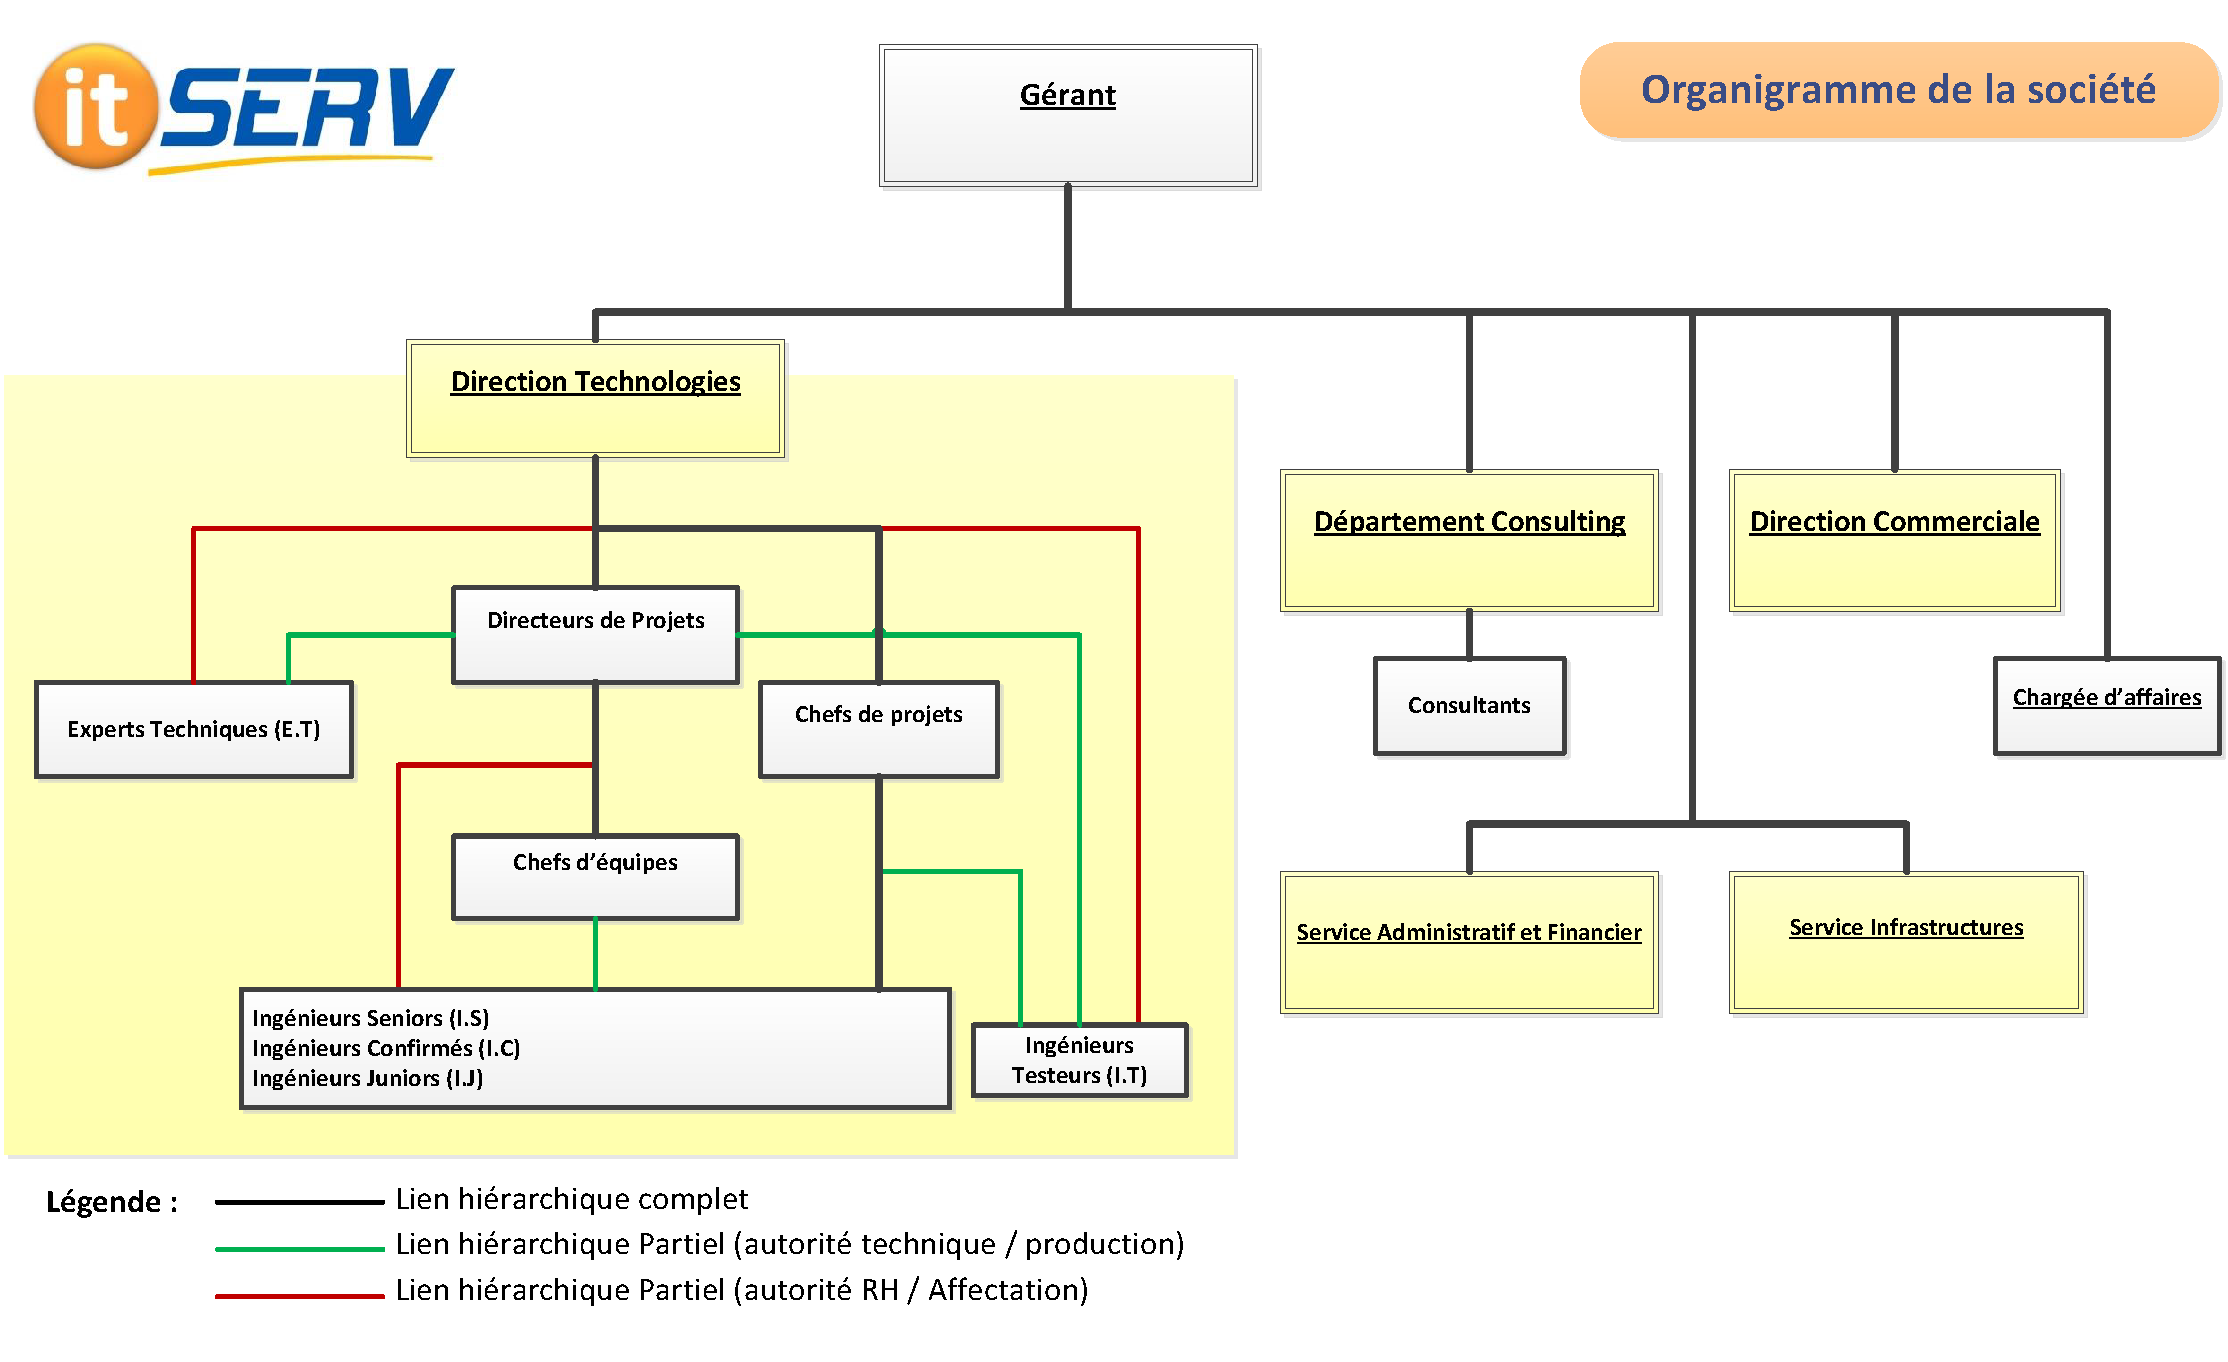
\includegraphics[scale=0.8]{organigramme.png}
\caption{Organigramme de l'entreprise}
\label{organigrammeImg}
\end{figure} 

\subsection{Domaine d'expertise}
Elle est sp�cialis�e dans la d�finition, la conception et l'appropriation des espaces. "UrbaProd" est pr�sente tout  au long du cycle de vie du processus d'optimisation et de conception des lieux afin d'am�liorer la disposition  des collaborateurs :
\begin{itemize}
                                 \item En amont pour le recueil des besoins et le cadrage strat�gique.
                                 \item Puis pour la conception et la r�alisation des plans des espaces.
                                 \item Enfin pour la gestion et le pilotage de mobilit� et l'ing�nierie de transfert.
                               \end{itemize}
Les missions de "UrbaProd" incluent :
\begin{itemize}
  \item Audit et programmation - Concept et charte d'am�nagement - Etudes et space planning.
  \item Prospective - Management de projet - Conduite du changement.
  \item Architecture d'int�rieur - Prescription mobilier - Conduite de travaux.
  \item Pilotage et gestion de la mobilit� - Ing�nierie de transfert.
  \item Solutions num�riques de gestion et visualisation des espaces.
\end{itemize}
"UrbaProd" travaille et accompagne les processus d'am�nagements des grands comptes en France et en Europe, � savoir : EDF, Thales, Cartier, Danone, INPI, l'Or�al, Technicolor, Hachette Livre dont nous retrouvons les logos dans la figure \ref{refenrenceImg}.

\begin{figure}[!ht]
\centering

\includegraphics[scale=0.8]{reference.png}
\caption{R�f�rences de l'entreprise}
\label{refenrenceImg}
\end{figure}

\section{Probl�matique}
Aujourd'hui, nous avons de plus en plus de demandes � traiter, sans avoir un support informatique pour les g�rer. Ce n'est pas tr�s ais� de g�rer l'historique de la client�le d'une entreprise. De plus, lors des diff�rentes int�ractions avec la client�le, et en particulier lors du partage d'informations, l'outils utilis� est le mail. Cependant, cela vire au d�sordre, i.e. messages dissparus, m�thodes de classements qui diff�rent d'un collaborateur � un autre, absence de suivi. Et comme la relation entre collaborateurs est la priorit� strat�gique de la soci�t�, ce point est � travailler d'urgence.

\section{Solutions existantes}
Il existe plusieurs solutions de gestion de relation client sur le march�. En examinant ces applications, nous citons les plus importantes :
\subsection{Version �diteur}
\begin{itemize}

\item[\ding{108}]
\textbf{CRM de Fitnet Manager} : Fitnet Avant-vente est l'outil de gestion commerciale de Fitnet Manager. Les solutions CRM et ERP existent c�tes � c�tes. Activ�es ensemble, elles fonctionnent d'une mani�re enti�rement int�gr�e. Fitnet Manager couvre ainsi l'ensemble du cycle de vie de l'activit� : depuis la prospection jusqu'� la facturation et l'analyse dans les reporting \cite{Fitnet}.

  \item[\ding{108}]
  \textbf{Everwin CXM} : c'est une solution qui vise les cabinets d'architectures, elle couvre plusieurs fonctionnalit�s citant � titre d'exemple :
  \begin{itemize}
    \item
    Base de donn�es de la soci�t� et des contacts avec gestion automatis�e de la t�l�prospection.
    \item
    Gestion des actions commerciales et des campagnes marketing.
    \item
    Agenda partag� et planning g�n�ral des collaborateurs.
  \end{itemize}

\end{itemize}
Cette solution est fond�e sur une technologie Client/Serveur sous windows avec une base de donn�es SQL Server.
il est disponible en mode SaaS ou licence et peut �tre coupl� aux ERP ERPEverwin SX et Everwin GX \cite{Everwin} .   La figure \ref{everwinImg} illustre l'ensemble des fonctionnalit�s couvertes par Everwin CXM.

\begin{figure}[!ht]\centering
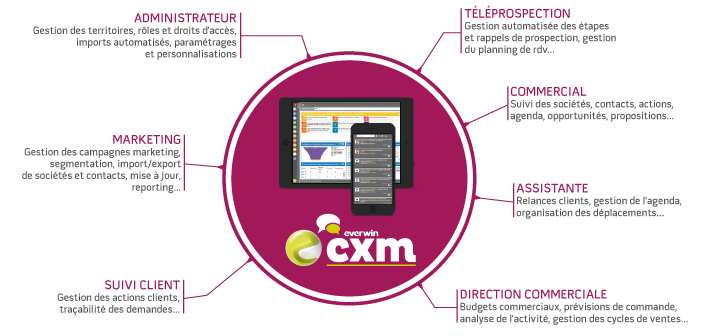
\includegraphics[scale=0.9]{everwinCXM.png}
\caption{Fonctionnalit�s offertes par Everwin CXM \cite{Everwin} }
\label{everwinImg}
\end{figure}

\subsection{Version libre}
 \textbf{Dolibar ERP/CRM} : cette solution g�re les activit�s professionnelles ou associatives de point de vue contact, commandes, stock. Elle g�re aussi la gestion des projets et les avancements de leurs t�ches, et assure m�me la gestion de la ressource humaine.
	Dolibarr est disponible pour toute plate-forme puisqu'elle est d�velopp�e en PHP, MySQL ou encore PostgreSQL .
La figure \ref{dolibarr1Img} illustre l'architecture sur laquelle est bas�e la solution Dolibarr :

\begin{figure}[!ht]\centering
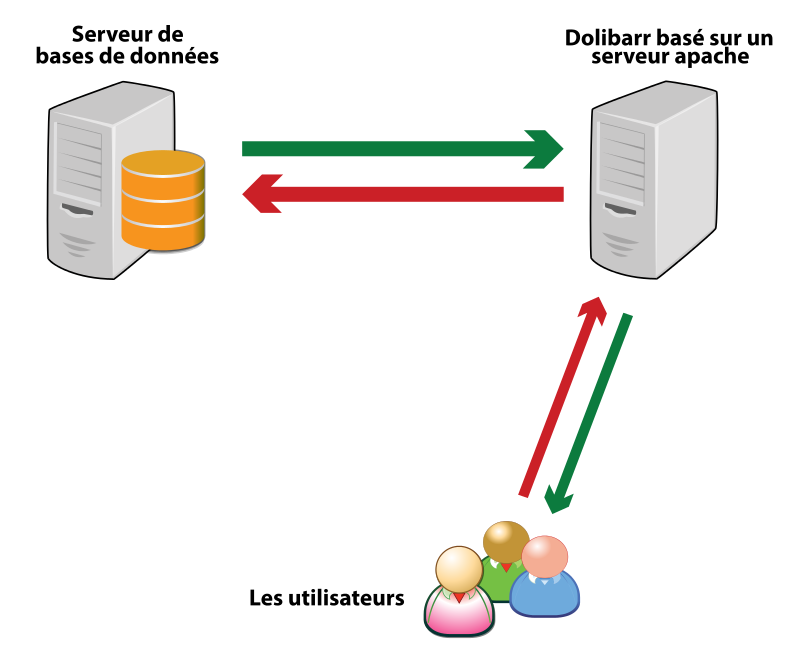
\includegraphics[scale=0.4]{Dolibarr1.png}
\caption{Architecture Dolibarr \cite{Dolibarr} }
\label{dolibarr1Img}
\end{figure}

Pour les non connaisseurs dans le domaine du d�veloppement, il existe un auto-installateur qui se charge d'installer la solution avec tous ses pr�-requis (apache,mysql,php) \cite{Dolibarr}.
La figure \ref{dolibarr2Img} pr�sente l'�cran d'accueil de Dolibarr :

\begin{figure}[!ht]\centering
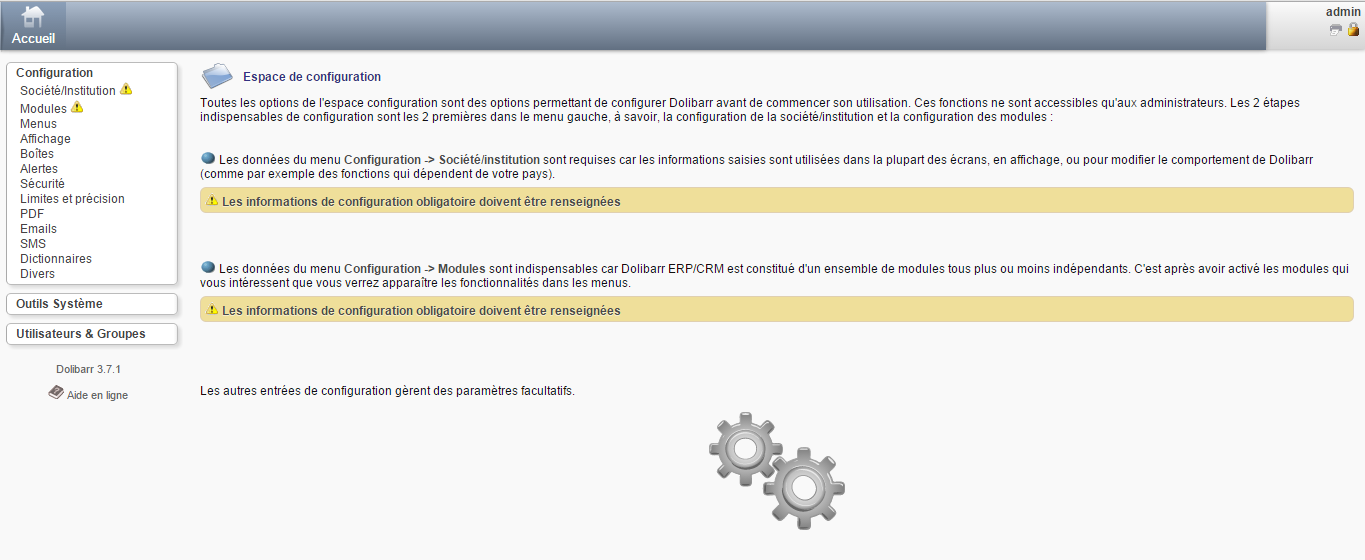
\includegraphics[scale=0.5]{accueil.png}
\caption{Ecran d'accueil de Dolibarr \cite{Dolibarr} }
\label{dolibarr2Img}
\end{figure}

\subsection{Etude comparative}
Le tableau \ref{compSolExt} pr�sente un comparatif entre les solutions existantes pr�sent�es pr�c�demment :

\begin{table}[!ht]\centering
  \centering
  \begin{tabular}{|c|c|c|c|c|c|}
    \hline
    % after \\: \hline or \cline{col1-col2} \cline{col3-col4} ...
    Solution & Payante &  Commentaire & Alertes & Mails & Accueil simple \\
    \hline
    Fitnet & oui  & non & oui & oui & non \\
    \hline
    Everwin CXM & oui  & non & oui & oui & non \\
    \hline
    Dolibarr & non  & non & oui & oui & non \\
    \hline
  \end{tabular}
  \caption{Comparatif entre les solutions existantes}\label{compSolExt}
\end{table}

Les applications �tudi�es, qu'elles soient en versions �diteurs ou m�me gratuites, et malgr� leurs adaptabilit�s et la diversit� de leurs fonctionnalit�s offertes, restent incapable de satisfaire les exigences de la soci�t�. En effet, elles n'int�grent pas un syst�me de commentaire et leur manipulation reste plut�t complexe compar�e � la solution � laquelle nous voulons aboutir.

\section{Objectifs du projet}
Nous voulons offrir un meilleur service dans nos r�ponses aux collaborateurs � l'aide d'un v�ritable outil de gestion des demandes. Aujourd'hui nous visons de :
\begin{itemize}
  \item Faciliter la gestion des demandes.
  \item Rendre l'interaction entre les collaborateurs situ�s en Tunisie et en France plus fluide.
  \item Avoir un syst�me de notification dans l'application, par mail et par sms.
  \item Mesurer leur taux de satisfaction vis-�-vis des r�ponses aux demandes.
  \item Identifier le dysfonctionnement dans notre processus de travail.
  \item Avoir un suivi et une �valuation.
\end{itemize}

\section{Contexte m�thodologique du projet}
La grande �volution dans le domaine du d�veloppement est accompagn�e par une �volution des moyens assurant le bon fonctionnement de ce dernier. D'o� l'apparition des m�thodes agiles permettant d'organiser le cycle de d�veloppement des projets informatiques.

Les m�thodes agiles sont bas�es sur des principes communs d�finis dans l'Agile Manifesto qui est r�dig� par des experts dans ce domaine \cite{AgManifesto}. Ils se reposent essentiellement sur une approche it�rative incr�mentale et adaptative �voluant en parall�le avec les besoins du client, afin de livrer un produit de qualit�.
Il existe plusieurs m�thodes agiles, � savoir, la m�thode  RUP \cite{RUP}, la m�thode XP \cite{XP}, la m�thode SCRUM \cite{SCRUM} et la m�thode RAD \cite{RAD}.

\subsection{Le choix de la M�thode Scrum}
Dans la majorit� des projets, il est difficile d'anticiper les attentes du client. Ceci nous oriente vers une approche it�rative permettant de s'adapter aux exigences du client au fur et � mesure de l'avancement du projet. Pour ce faire, nous avons choisi d'adopter la m�thode Scrum.
Aujourd'hui, Scrum est la m�thode agile la plus utilis�e. Elle permet de produire une solution de la plus haute qualit� dans des bref d�lais.
Cette m�thode est munie des atouts suivants :
\begin{itemize}
  \item Meilleur vue d'ensemble du projet : nous avons une vue globale sur l'avancement du projet par tous les membres des diff�rentes �quipes avec un traitement r�gulier des probl�mes rencontr�s durant chaque phase.
  \item Mise � jour des priorit�s : le client, qui n'est pas n�cessairement un informaticien, n'a pas toujours une vision compl�te sur le produit final. Pour cela, et gr�ce � la composition s�quentielle du contenu des sprints, il b�n�ficie d'une flexibilit� au niveau de la d�finition, de l'�volution des priorit�s et des s�quences d'activit�s.
  \item Qualit� du produit mise en avant : Cette m�thode se repose sur une �valuation r�guli�re du travail, ce qui permet un meilleur traitement des probl�mes (bug), une meilleure productivit� et un produit satisfaisant \cite{AvantageScrum}.
\end{itemize}

\subsection{Les r�les et les notions}
Les r�les dans Scrum :
\begin{itemize}
  \item Le product owner est le responsable du produit. Il est g�n�ralement le client et c'est lui qui exprime les diff�rentes sp�cifications fonctionnelles et leurs priorit�s.
  \item L'�quipe de d�veloppement est responsable de la r�alisation du livrable. Elle est constitu�e par l'entreprise et elle est auto-organis�.
  \item Le scrum master est le premier responsable sur le bon d�roulement des processus de la m�thode scrum.
\end{itemize}

Notion :
\begin{itemize}
  \item Sprint  : une it�ration de travail qui dure entre 15 et 30 jours.
  \item Le product backlog : repr�sente la liste des fonctionnalit�s r�dig�es par le product owner avec tous les correctifs et les am�liorations. Il est donc modifiable tout au long du projet. Le product backlog est pr�sent� sous forme d'items.
  \item Le sprint backlog : est l'ensemble des items planifi�s pour le sprint en cour \cite{SCRUM}.
\end{itemize}


\section*{Conclusion}
Dans ce chapitre, nous avons pr�sent� le cadre g�n�ral du travail, en commen�ant par la pr�sentation de l'entreprise Urbaprod, passant par la probl�matique du projet, ainsi qu'une �tude des solutions existantes sur le march�. Et pour finir, nous avons pr�sent� la m�thode qui va guider notre travail tout au long du projet. Dans le chapitre suivant, nous introduisons les sp�cifications de notre projet.


%==============================================================================
\end{spacing}

\setcounter{chapter}{1}
\chapter{          ÉTUDE PRÉLIMINAIRE}
\minitoc %insert la minitoc
\graphicspath{{Chapitre2/figures/}}

%\DoPToC

%==============================================================================
\pagestyle{fancy}
\fancyhf{}
\fancyhead[R]{\bfseries\rightmark}
\fancyfoot[R]{\thepage}
\renewcommand{\headrulewidth}{0.5pt}
\renewcommand{\footrulewidth}{0pt}
\renewcommand{\chaptermark}[1]{\markboth{\MakeUppercase{\chaptername~\thechapter. #1 }}{}}
\renewcommand{\sectionmark}[1]{\markright{\thechapter.\thesection~ #1}}

\begin{spacing}{1.5}

%==============================================================================
\section*{Introduction}
Après avoir présenté le cadre général de notre projet, nous entamons par le biais de ce chapitre une étude théorique, préface à sa réalisation. Nous commençerons par présenter les notions de base associées à la partie métier du projet. Nous enchaînerons avec l'étude de l'existant, qui sera l'opportunité de présenter plus en détail la problématique rencontrée en interne par l'entreprise. Enfin, une vue d'ensemble des solutions similaires présentes sur le marché permettra de se faire une idée globale sur les fonctionnalités à attendre du produit.\\
Cette étude, partie intégrale de l'élaboration de la vision initiale du produit, s'inscrit dans la phase d'inception de la méthodologie de travail adoptée.


%==============================================================================
\section{La Gestion de Projet}
Les entreprises se confrontent à de nombreux challenges au cours de leur évolution (adaptation à des contraintes externes, lancement de nouveaux services ou produits, intégration de nouveaux outils, mises à jour des processus, ...). Chaque défi est relevé sous forme de projet. Un projet est défini sous forme d'une suite d'actions délimitée dans le temps, en vue de produire un résultat spécifique, un produit, un service ou une nouvelle organisation.\\
La gestion de projet a pour vocation de relever ces défis en mettant en place une organisation et une planification de l’ensemble des activités visant à assurer l’atteinte des objectifs du projet (qualité, coûts, délais, ...), à effectuer leur suivi, anticiper les risques et les changements à mettre en œuvre  ainsi qu'à gérer la communication et la prise de décision.\\
\\
On peut regrouper les activités de gestion de projet en deux phases :
\begin{itemize}
%    \item \textbf{} :
    \item La phase d'organisation
    \item La phase de pilotage
\end{itemize}
\\
Ces activités sont précédées par une phase de collecte d'informations et d'étude de faisabilité. Cette phase d'avant projet permet de valider le projet et de décider des ressources à mobiliser pour sa mise en œuvre.
% REF: http://ressources.aunege.fr/nuxeo/site/esupversions/6b35be1e-5317-4cd6-8db2-05485615219d
% REF: http://www.gestiondeprojet.net
%-----------------------------------------------------------------------------------
\subsection{Phase d'organisation}
La phase d'organisation comprend le développement des concepts définis dans la phase d'avant projet et la définition du référentiel du projet, en fournissant suffisamment de détails pour pouvoir entamer la phase de réalisation. Les principaux éléments du référentiel d'un projet incluent :
\begin{itemize}
%    \item \textbf{} :
    \item \textbf{La charte du projet} : Elle est rédigée par le chef de projet dès son lancement. Elle est destinée à toutes les personnes appelées à travailler sur le projet, ainsi qu'aux tiers concernés (la hiérarchie, les chefs de service, ...). C'est un document de référence à usage strictement interne dont le but est de fournir les informations de base du projet : son objet, ses parties prenantes, ses enjeux, ses contraintes, etc.
    \item \textbf{La structuration du projet} : La structure de découpage du projet organise et définit la totalité du contenu d'un projet. La structuration du projet dépend de nombreux paramètres (la complexité, la structure de l'organisation, le type de gestion, ...) et a pour objectif de découper le projet en plus petits éléments, plus faciles à gérer, afin de pouvoir définir des coûts et des durées pour chaque élément, ainsi que des résultats tangibles et mesurables.
    \item \textbf{Le planning de référence} : La planification d'un projet est l’activité qui consiste à déterminer et à ordonnancer les tâches du projet, à estimer leurs charges et à déterminer les profils nécessaires à leur réalisation. Le planning résultant inclut la liste des tâches et leurs antériorités, la définition des lots de travaux ainsi que les ressources associées.
    \item \textbf{Le plan de communication} : C'est un document qui présente les méthodes et les modalités adoptées pour collecter, conserver et diffuser l'information, les destinataires de chaque type d'information (rapport, document technique, ...), ainsi que les responsabilités associées.
    \item \textbf{Le budget de référence} : Résultat de l'analyse des coûts rattachés au projet, il est établi à partir de la liste des activités, des ressources associées et du planning de référence.
    \item \textbf{L'analyse des risques} : Elle comporte un recensement des aléas majeurs associés au projet ainsi que les plans d'action et les mesures préventives à mettre en place.
\end{itemize}

%-----------------------------------------------------------------------------------
\subsection{Phase de pilotage}
Une fois budgétisé, organisé et planifié, le projet démarre. Le pilotage du projet permet de comparer le réalisé avec le prévisionnel, et de réviser éventuellement les plannings et les charges. Le chef de projet et son équipe s'efforcent de respecter le référentiel de gestion du projet, tout en mesurant les écarts constatés. Cela inclut la maîtrise des aspects suivants :
\begin{itemize}
%    \item \textbf{}} :
    \item \textbf{Les délais} : Le chef de projet recueille l'information sur l'avancement réel du projet à partir de l'avancement de chaque tâche, et identifie les retards actuels et potentiels. Dès lors, des actions correctives peuvent être mises en place afin de corriger les écarts (modification du planning, réallocation de ressources, ...).
    \item \textbf{Les coûts} : Une évaluation de la consommation budget est fréquemment entreprise, suivie d'une réestimation du budget qui reste à consommer. Le coût total prévu comparé au budget de référence permet d'analyser et d'anticiper des écarts ainsi que d'identifier les causes de dépassement.
    \item \textbf{Les modifications} : Elles sont le résultat d'événements extérieurs (changement de réglementation, changement demandé par le client, erreurs ou oublis dans la définition initiale, ...). Les demandes de changements peuvent apparaître sous plusieurs formes et conduire à un élargissement ou à une limitation du contenu et doivent être traitées grâce un ensemble de procédures formelles.
    \item \textbf{Les risques} : La maîtrise des risques permet d'identifier, de quantifier, de réduire ainsi que de suivre les risques encourus tout au long de la vie du projet.
\end{itemize}
Le chef de projet se focalise essentiellement sur la maîtrise des coûts et des délais.\\

L'usage d’indicateurs de pilotage est crucial pour le pilotage efficace d'un projet. Ces outils d'assistance à la décision permettent de mesurer de manière pratique une situation ou un risque, d'alerter ou au contraire de signifier l'avancement correct d'un projet.


%==============================================================================
\section{Étude de l'existant}
L'étude de l'existant permet d'identifier les points forts ainsi que les points faibles de la solution existante. Cette étude permettra de bien cibler les besoins de l'entreprise, en vue d'en tenir compte lors de la conception et du développement de la solution.
%-----------------------------------------------------------------------------------
\subsection{Description de l'existant}
La solution de gestion de projet actuelle se base sur l'utilisation du logiciel Excel pour générer des documents associés aux différentes activités d'un projet. En effet, le chef de projet répertorie chaque catégorie d'artéfact associée à la gestion d'un projet sous forme de tableur Excel. Il procède ainsi à l'ajout et l'édition d'entrées pour chaque catégorie d'artéfact et y indique l'ensemble des informations requises. Cette procédure est facilitée par la duplication de fiches Excel de base, vierges, préparées à l'avance pour chaque catégorie. Ainsi, pour chaque catégorie d'artéfact, l'ensemble des entêtes et des valeurs prédéfinies pour chaque champs y est déja déclaré. La table d'entrées d'une fiche est souvent accompagnée d'un ensemble d'indicateurs, statiques et dynamiques, pertinents à la catégorie en question. Des exemples de ces fiches sont exposés aux figures \ref{fig:risqueFiche} et \ref{fig:actionFiche}, traitant respectivement des artéfacts actions et risques pour un projet.

\begin{figure}[H]
\centering
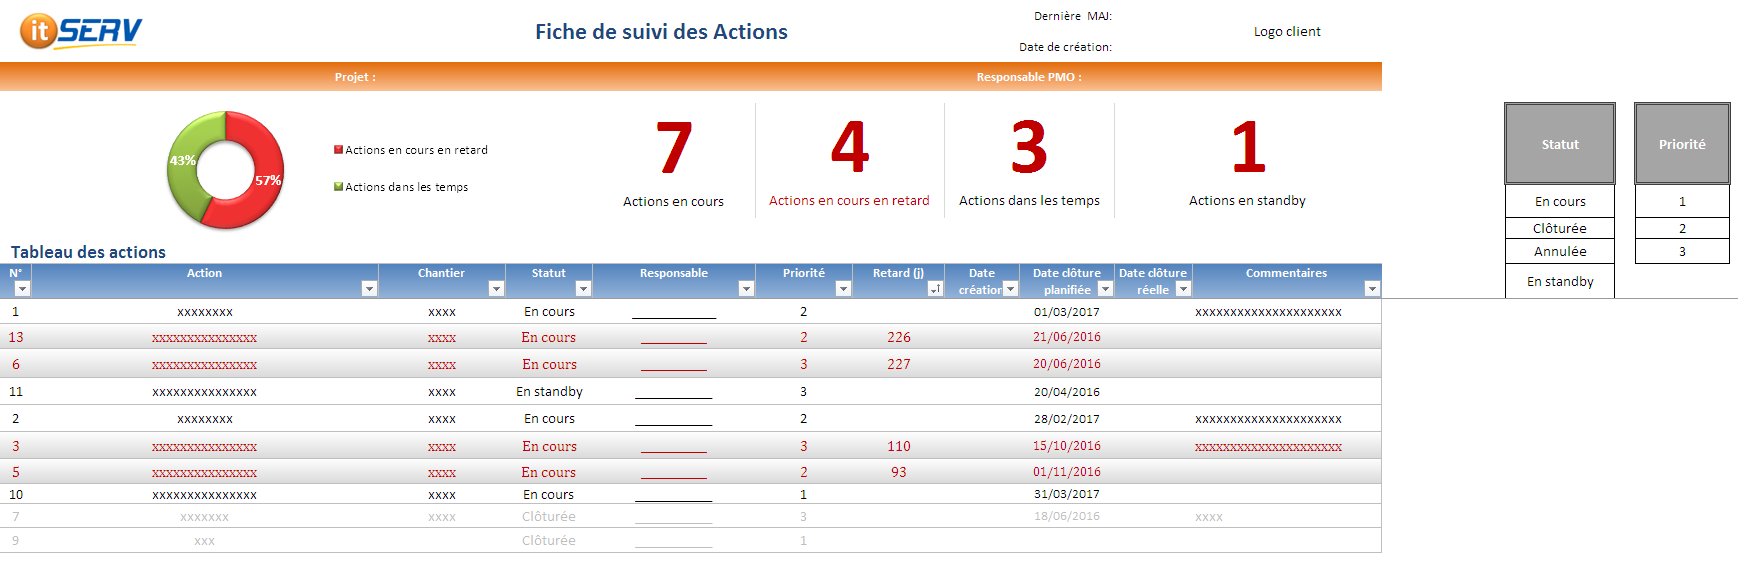
\includegraphics[width=\linewidth]{ficheActions.png}
\caption{Exemple d'une fiche de suivi des actions}
\label{fig:actionFiche}
\end{figure}

\begin{figure}[H]
\centering
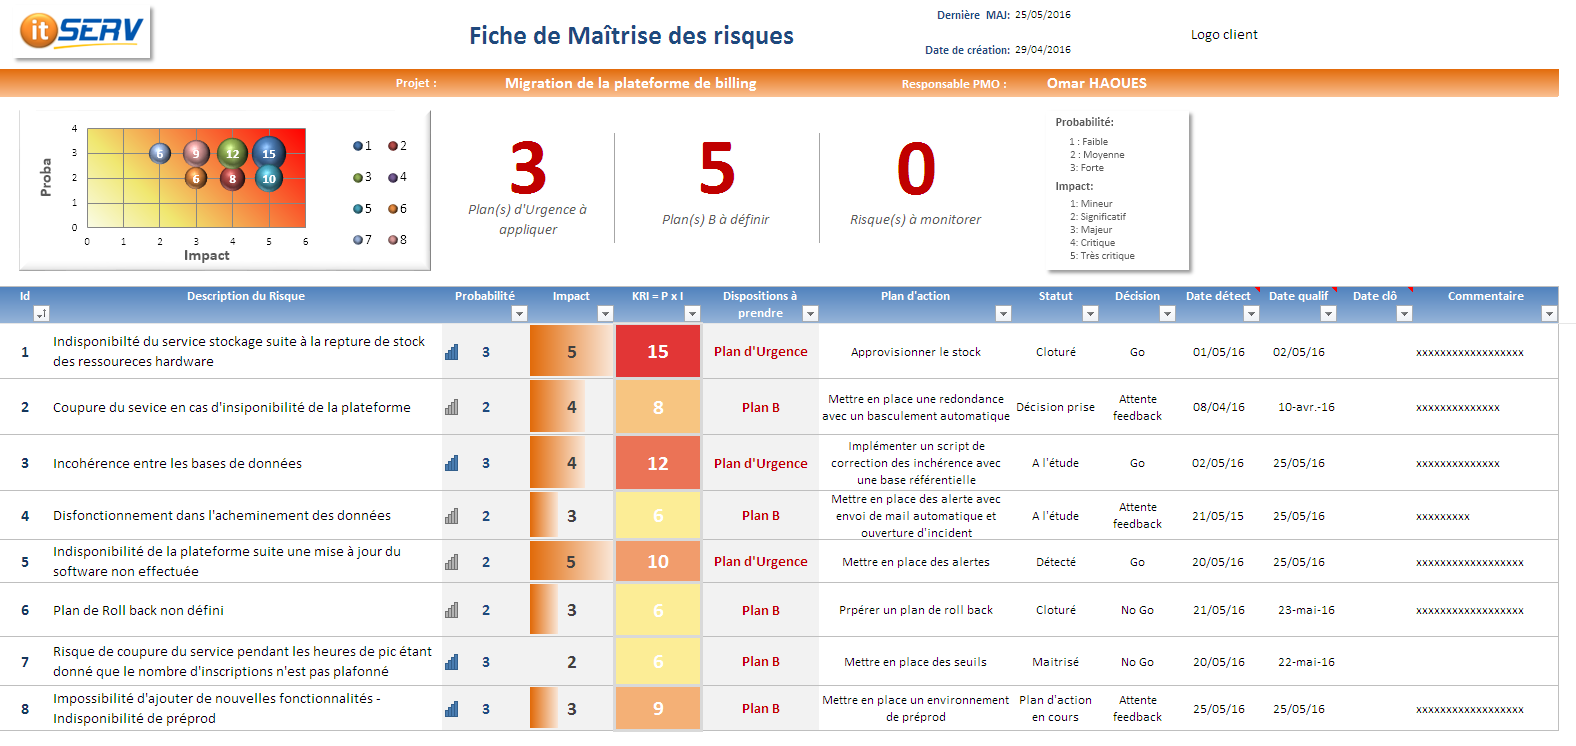
\includegraphics[width=\linewidth]{ficheRisques.png}
\caption{Exemple d'une fiche de maîtrise des risques}
\label{fig:risqueFiche}
\end{figure}
\

Le chef de projet est régulièrement chargé de diffuser les mises à jour relatives à un projet, périodiquement ou à la demande, au travers de l'envoi de messages électroniques directement aux parties concernées.\\

Cette méthode de travail possède certains atouts, mais dissimule dans l'ensemble plusieurs inconvenances qui nuisent à son niveau d'efficacité et à la performance de la gestion de projets par l'entreprise. Ces points sont exposés dans la section suivante.

%-----------------------------------------------------------------------------------
\subsection{Critique de l'existant}
La présentation de la méthode de gestion actuelle nous permet de déceler des limitations importantes, inhérentes à la démarche générale.\\
\\
Reconnaissons tout d'abord les mérites non négilgeables de celle-ci, à savoir :
\begin{itemize}
    \item Disponibilité de fiches de base, contraignant les champs à choix restraints aux options prédéfinies et assistant à leur remplissage
    \item Présence de champs autocalculés ainsi que de supports visuels utiles pour la compréhension de certains champs, dont la signification peut s'avérer obscure
    \item Génération automatique d'indicateurs riches (statistiques numériques, graphiques en camembert, ...)
\end{itemize}
\

Outre ces quelques bénéfices, cette méthode de gestion présente les nombreuses limitations suivantes :
\begin{itemize}
    \item \textbf{Perte en productivité} : induite d'un déficit d'automatisation de la démarche de gestion des fichiers
    \item \textbf{Fragmentation des données} : les données relatives à chaque projet sont réparties, sous forme d'une multitude de documents, souvent désorganisés
    \item \textbf{Journalisation non fiable des mises à jour} : la journalisation des mises à jours relève entièrement de l'organisation choisie par le chef de projet, et requiert un effort manuel, exclusivement dédié à la tâche
    \item \textbf{Traçabilité impossible} : l'origine des modifications des fichiers n'est pas connue
    \item \textbf{Stockage inneficace} : problème de centralisation pour l'ensemble des données des projets menés par l'entreprise, redondance de données, oraganisation manuelle, etc
    \item \textbf{Sécurité non garantie} : la sécurisation des données (documents) est entièrement à la charge des parties prenantes y ayant accès
    \item \textbf{Condifentailité difficile à assurer} : elle implique en pratique l'édition soigneuse, au cas par cas, des fichiers partagés
    \item \textbf{Synthèse des données impossible} : impossible de se reposer fiablement sur les données des fichiers pour les besoins d'aide à la décision de l'entreprise (à cause des points susmentionnés)
    \item \textbf{Collaboration fastidieuse} : contribution d'intervenants non gérée par la solution actuelle. Le chef de projet transforme individuellement tous les flux d'information en données, avant de les indiquer dans le fichier approprié
\end{itemize}
\

Toutes les limitaions susmentionnées imposent pour l'entreprise une révolution dans sa méthode actuelle de gestion de projets. Dans le cadre de notre projet de fin d'études, la solution à concevoir aspire ainsi à combiner les points forts de la démarche existante tout en apportant une solution efficace à ses problèmes inhérents.


%==============================================================================
\section{Étude des solutions existantes sur le marché}
Le problème de gestion de projet est aussi vieux que le concept de projet lui-même. En conséquence, un nombre important de solutions logicielles d'aide à la gestion de projet est disponible aujourd'hui sur le marché. Dans le but de produire une solution de qualité, une étude de l'existant s'impose afin de prendre en considération les points forts et les points faibles des solutions existantes. Celle-ci servira surtout à nous guider dans l'élaboration de la vision de notre produit.

%-----------------------------------------------------------------------------------
\subsection{Présentation des solutions existantes}
Les solutions présentes sur le marché se distinguent les unes des autres essentiellement par le niveau de fonctionnalités offert et le domaine d'application cible. En effet, des solutions populaires, telle que JIRA \ref{JIRA}, se limitent à un domaine très particulier, en l'occurence la gestion de projets agiles pour cette dernière. Les solutions étudiées aspirent à être le plus générique possible, capable d'être employées dans n'importe quel contexte de projet. L'échantillon exposé ci-dessous vise à présenter une vue d'ensemble des caractéristiques communes et distinctives des solutions les plus populaires sur le marché qui partagent cette vision.

\subsubsection*{MS Projects} %-------------------------------------------------------------------------
Microsoft Projects a su s'imposer pendant longtemps en tant que solution de facto pour les besoins de gestion de projet en entreprise. Faisant partie de la suite logicille de l'éditeur, MS Projects ne fait pas exception et s'intègre pleinement à sa plateforme collaborative \ref{Office 365}, ce qui représente un réel bénéfice pour les clients ayant déja opté pour l'intégration de leurs données sur cette dernière. Le logiciel continue d'introduire un nombre de fonctionnalités avancées avec ses mises à jour. Ceci le rend particulièrement adapté aux besoins poussés de gestion de projet. Les utilisateurs expérimentés y trouvent leur compte, cependant la courbe d'apprentisage est souvent pénible pour les novices et s'avère être trop complexe pour les usages se limitant en besoin à un nombre restreint de ses fonctionnalités.

\subsubsection*{ProjectManager.com} %------------------------------------------------------------------
ProjectManager.com couvre très bien les fonctionnalités de base de gestion de projet et, parmi toutes les solutions étudiées, s'apparente le plus à la vision initiale élaborée. Cette solution, disponible sous une offre SaaS \ref{SaaS}, s'adapte parfaitement aux besoins des petites et moyennes entreprises, qui retrouvent une simplicité d'usage associée à une couverture plus que décente des piliers de la gesion professionnelle de projet.

\subsubsection*{Zoho Projects} %-----------------------------------------------------------------------
Zoho propose une suite logicielle qui répond aux besoins des particuilers et des entreprises. Dans cette optique, sa solution de gestion de projet s'intègre parfaitement avec certains de ses autres produits, afin d'étendre ses fonctionnalités. La solution se veut simple, mais complète, en offrant un éventail éttoffé de fonctionnalités pour la gestion des divers facettes d'un projet. Elle se caractérise par une attention particuière apportée à l'ergonomie et au confort général d'utilisation.

\subsubsection*{EasyProject (EasyRedmine)} %-----------------------------------------------------------------------------
Redmine est la solution open source gratuite la plus complète disponible sur le marché. Cependant, son manque d'intuitivité et le faible niveau d'ergonomie offert, associés à son interface datée, nuisent à son potentiel et en font une solution peu courante d'usage dans la pratique. C'est tout d'abord dans le but d'accroître son utilisabilité, tout en prenant avantage de la base de fonctionnalités existante, que la solution EasyProject offre une version commerciale, basée sur cette solution. Depuis, l'application s'est vu évoluer vers l'une des solutions les plus abouties du marché, visant à s'aligner avec les standards de gestion de projets IPMA et PMI.

\subsubsection*{Clarizen} %-----------------------------------------------------------------------------
Due à l'amélioration continue de son produit et à la complétude de sa vision, l'entreprise Clarizen a vu son produit se hisser à la position de Leader dans dans les classements Gartner et Forrester de 2016 \ref{clarizen.com}, dans la catégorie des solutions SaaS de gestion de projets. De ce fait, ce produit a sans nul doute sa place dans notre étude et impose un bilan des traits caractéristiques qui lui valent son succès.
\\

Dans le but de présenter un échantillon pertinent, d'autres solutions ont été omises, notamment pour des raisons de redondance ou de pauvreté en termes de fonctionnalités. Nous poursuivons avec la mise en relief des points communs et distinctifs de chacune dans la partie qui suit.

%-----------------------------------------------------------------------------------
\subsection{Synthèse des solutions existantes}

Le tableau \ref{tab:} présente une comparaison haut niveau des solutions étudiées. On y observe que les solutions retenues partagent un tronc commun de fonctionnalités destiné à la gestion des aspects primordiaux d'un projet. Elles se différencient néanmoins sur d'autres points, tel que la nature de l'offre et le support de l'accès mobile.

\begin{table}[h]
\centering
\caption{Comparatif des solutions de gestion de projet présentées}
\label{comparatifSolutionsEtudiees}
\begin{tabularx}{1\textwidth}{|p{4cm}|1|1|1|1|1|}
\hline
        \textbf{Spécificités} & \textbf{MS Proj.} & \textbf{P.M .com} & \textbf{Zoho Proj.}&  \textbf{EasyProject} & \textbf{Clarizen}\\
\hline
        \textbf{Nature d'offre} & Bureau & SaaS & SaaS & SaaS \& Local & SaaS\\
\hline
		\textbf{Planification} & \cmark & \cmark & \cmark & \cmark & \cmark\\
\hline
		\textbf{Gestion Budget} & \cmark & \cmark & \cmark & \cmark & \cmark\\
\hline
		\textbf{Structuration} & \cmark & \cmark & \cmark & \cmark & \cmark\\
\hline
		\textbf{Gestion Ressources} & \cmark & \cmark & \cmark & \cmark & \cmark\\
\hline
		\textbf{Gestion Problèmes} & \cmark & \cmark & \cmark & \cmark & \cmark\\
\hline
        \textbf{Gestion} & \multirow{2}{*}{\xmark} & \multirow{2}{*}{\cmark} & \multirow{2}{*}{\cmark} & \multirow{2}{*}{\cmark} & \multirow{2}{*}{\cmark}\\
        \textbf{Modifications} &  &  &  &  & \\
\hline
		\textbf{Reporting} & \cmark & \cmark & \cmark & \cmark & \cmark\\
\hline
		\textbf{GED} & \cmark & \cmark & \cmark & \cmark & \cmark\\
\hline
		\textbf{Pilotage Risques} & \cmark & \cmark & \cmark & \cmark & \cmark\\
\hline
		\textbf{Support Mobile} & \xmark & Web & App & App & App\\
\hline
		\textbf{Collaboration} & \xmark & \cmark & \cmark & \cmark & \cmark\\
\hline
		\textbf{Open Source} & \xmark & \xmark & \xmark & \cmark & \xmark\\
\hline
\end{tabularx}
\end{table}
\

Vu son expertise en développement d'applications, IT SERV a choisi de démarrer le développement de sa propre solution d'aide à la gestion de projet. Dans le cadre de notre projet de fin d'études, nous visons à concevoir une solution s'inspirant d'une sélection des traits jugés primordiaux des solutions étudiées. Ceux-ci seront établis dans le chapitre \ref{chap: spécs}.

%==============================================================================
\section*{Conclusion}
Afin de mieux cerner la problématique et de proposer une solution de qualité, tenant compte des spécificités de notre projet, nous avons établi l'état des lieux de l'existant, que ce soient les méthodes de gestion courantes de l'entreprise, ou les solutions similaires disponibles sur le marché.\\
Avec ces informations en main, le chapitre suivant nous permettra de dégager précisément les exigences de notre produit.


%==============================================================================
\end{spacing}

\setcounter{chapter}{2}
\chapter{PRÉPARATION AU LANCEMENT}
\minitoc %insert la minitoc
\graphicspath{{Chapitre3/figures/}}

%\DoPToC

%==============================================================================
\pagestyle{fancy}
\fancyhf{}
\fancyhead[R]{\bfseries\rightmark}
\fancyfoot[R]{\thepage}
\renewcommand{\headrulewidth}{0.5pt}
\renewcommand{\footrulewidth}{0pt}
\renewcommand{\chaptermark}[1]{\markboth{\MakeUppercase{\chaptername~\thechapter. #1 }}{}}
\renewcommand{\sectionmark}[1]{\markright{\thechapter.\thesection~ #1}}

\begin{spacing}{1.5}

%==============================================================================
\section*{Introduction}
Avant d'appréhender le développment du système, il est primordial d'acquérir une compréhension claire des besoins des parties prenantes au projet, et des fonctionalités escomptées du système.\\
Ce chapitre couronne l'étape d'élaboration de la vision de notre produit, par la spécification des besoins. La phase d'inception se poursuit avec l'édification de l'architecture globale du produit et le choix de l'environnement technique. Ces deux parties conclueront le chapitre et annoncent l'achèvement de la phase d'inception.

%==============================================================================
\section{Analyse des besoins}
L'analyse des besoins a pour objectif l'identification des acteurs du système et de leurs rôles, ainsi que la spécification des besoins et des contraintes contre lesquelles le produit final sera validé. Il existe deux types de besoins :
\begin{itemize}
    \item Les besoisn fonctionnels, qui présentent ce que l'utilisateur attend en terme de service
    \item Les besoins non fonctionnels, qui présentent les contraintes sous lesquelles l'application doit être opérationnelle
\end{itemize}

%-----------------------------------------------------------------------------------
\subsection{Objet global du projet}
L'objectif du projet consiste à la conception, au développement, ainsi qu’au déploiement, d’une application web de gestion de projets, compatible avec tous les terminaux, de format réduit ou large, et disponible d’usage principalement en mode SaaS.\\
Pour toute organisation cliente, l’application permettra essentiellement aux responsables, chefs de projet, de gérer les différents aspects des projets entrepris par leur organisation, ainsi que d’en monitorer l’état.\\

Le produit final comportera ainsi deux parties distinctes :
\begin{itemize}
\item Une application web de gestion de projets en mode SaaS, ou à déploiement en interne
    \item Une solution complémentaire pour la gestion de l’aspect SaaS
\end{itemize}

%-----------------------------------------------------------------------------------
\subsection{Identification des acteurs}
L’application est destinée à être acquise par une organisation de petite ou de grande envergure (entreprise, équipe, …). Au sein de celle-ci, nous pouvons distinguer entre trois types d'acteurs à rôles distincts pour notre système :
\begin{itemize}
    \item \textbf{L'administrateur} : C’est l'utilisateur associé au compte existant par défaut lors de l'acquisition de la solution. Il possède les pleins pouvoirs sur le reste des comptes et a la charge de créer le autres comptes au tout début de la mise en route de l'application.
    \item \textbf{Un chef de projet} : C’est l'utilisateur fondamental du système. Il s'intéresse essentiellement à l'aspect de gestion de projets mais garde la possibilité de créer des comptes utilisateurs, à plus faible ou égal pouvoir, et de les gérer à sa guise.
    \item \textbf{Un intervenant} : Cet utilisateur est généralement externe à l'organisation et a pour but de contribuer à la gestion d'un projet. Son compte est créé par un chef de projet, ou l'administrateur, lequel lui procure des droits d'accès à différentes parties d'un projet, son rôle se restraignant à intervenir sur ces parties.
    \item \textbf{Un dirigeant} : Cet utilisateur, généralement interne à l'entreprise, s'intéresse et se limite uniquement à l'exploitation des fonctionalités de reporting offertes par le système, pour l'ensemble du portefeuille de projets. Son compte est créé et géré par l'administrateur.
    \item \textbf{Une partie prenante} : Cet utilisateur se limite à l'exploitation des fonctionalités de reporting offertes par le système dans le cadre d'un projet. Son compte est créé et géré par un chef de projet.
\end{itemize}
\

Pour la solution complémentaire de gestion de l’offre SaaS, on reconnait un type seul acteur, à savoir : L'administrateur SaaS. C’est lui qui gère les clients de l’offre SaaS. Il a la charge de monitorer l’usage de l’application en mode SaaS et de remédier aux requêtes des clients.

%-----------------------------------------------------------------------------------
\subsection{Spécification fonctionnelles}
On énumère ici les différentes contraintes et besoins fonctionnels requis de la part du livrable final.\\
L’application doit être en mesure d’offrir les fonctionnalités suivantes :
\begin{itemize}
    \item \textbf{Gestion du portefeuille de projets} : L'ensemble des projets du client doit être regoupé sous un portefeuille, qui offre des fonctionalités d'ajout et d'édition d'un ou plusieurs projets.
    \item \textbf{Gestion de la charte d'un projet} : Il s'agit d'offrir à l'utilisateur la possibilité de fournir les détails relatifs à la charte d'un projet dès sa création, tout en gardant la possibilité d'en éditer le contenu à postériori.
    \item \textbf{Reporting au niveau projet} : Une vue d'ensemble de l'état global d'un projet doit être accessible au travers d'un tableau de bord, contenant un agencement d'indicateurs clés pour le pilotage d'un projet.
    \item \textbf{Gestion de l'intégration} : Un projet doit pouvoir être structuré sous les différents niveaux suivants : projet, sous projet et chantier. Un projet peut inclure un ensemble de sous projets ou de chantiers, directemnt ratachés à lui. Un sous projet existe uniquement sous un projet, et peut lui-même contenir une multitude de chantiers, lui étant directement associés.
    \item \textbf{Gestion du plan d'action} : Une action est une tâche à réaliser, disposant essentiellement d'une description, d'un responsable et d'une date de clôture planifiée. Une action doit pouvoir être rajoutée sous n'importe quel niveau d'un projet, et peut être mise à jour ou bien supprimée. Un indicateur sur les actions en retard sera mis à disposition.
    \item \textbf{Gestion des coûts} : Le budget d'un projet ou d'un sous projet peut être renseigné et mis à jour tout au long de son existance. La gestion du budget inclut la spécification du budget initial, du buget consommé ainsi que d'une estimation du budget qui reste à consommer. Elle offre par ailleurs un indicateur sur le budget total prévisonnel.
    \item \textbf{Gestion du reste à faire} : Un reste à faire se distingue par une description et une charge associée, en homme / jour. Les restes à faire peuvent être créés et mis à jour, et sont rattachables à n'importe quel niveau d'un projet.
    \item \textbf{Planification} : La planification d'un projet ou d'un sous projet sera possible au travers de la création et de la consultation ultérieure des principaux jalons du niveau de projet. En essence, un jalon est défini par une brève description associée à une date d'échéance.
    \item \textbf{Gestion du "Scope"} : La gestion du "scope" ou du périmètre d'un niveau de projet s'accomplit principalement via la fourniture de documents en pièces jointes au niveau en question. D'autre part, la gestion du périmètre couvre la gestion du changement et des points en suspens. Un point en suspens est un point relatif au niveau de projet, en attente de résolution, auquel un responsable est assigné. La gestion du changement quant à elle est formalisée au travers de la soumission de demandes de changement. Chaque demande inclut essentiellement le demandeur ainsi que la décision prise par rapport à celle-ci.
    \item \textbf{Gestion des risques} : Le définition des risques peut être réalisée à n'importe quel niveau d'un projet. Un risque est défini par une description du risque encouru, associée à une probabilité et un impact. Ces derniers sont utilisés pour générer un indicateur sur le niveau de criticité (KRI \ref{ANGRAMME}) du risque. Leur suivi est réalisé principalement au travers de la spécification du statut, du plan d'action et des dispositions à prendre pour chaque risque, ainsi que d'une date de qualification et une date de clôture.
    \item \textbf{Gestion des ressources humaines} : La définition des ressources humaines peut être réalisée au niveau du portefeuille global de projets ou bien au niveau d'un projet ou d'un sous projet. Les ressources globales peuvent plus tard être assignées à un projet en particulier. Au sein d'un projet ou d'un sous projet, les ressources humaines peuvent être renseignées, mises à jour, et éventuellement assignées à une action ou un point en suspens. Une ressource humaine peut également être assignée en tant que responsable d'un plan de communication au niveau d'un projet.
    \item \textbf{Gestion de la communication} : La gestion de la communication se déroule au sein d'un projet. Elle inclut la définition de plans de communication, se distinguant par une description et un responsable communication, de même que la planification de réunions, disposant chacune d'un nom, d'une date et d'un lieu, acoompagnés d'un statut, ainsi que des comptes rendus de réunions.
    \item \textbf{Gestion des ressources non humaines} : Toute ressource matérielle ou immatérielle associée à un niveau de projet doit pouvoir être renseignée et mise à jour.
    \item \textbf{Publication de mises à jour} : L'état d'un projet doit pouvoir être archivé sous forme d'une mise à jour.
\end{itemize}
\

D'autre part, la solution adjointe de gestion du service SaaS devra quant à elle permettre de gérer les clients de l'offre SaaS : création d’un client, mise à jour des détails associées à un client et gestion du compte administrateur attaché.

%-----------------------------------------------------------------------------------
\subsection{Spécification non fonctionnelles}
En plus d’apporter les fonctionnalités citées précédemment, le produit final devra être en mesure d'assurer les aspects suivants :
\begin{itemize}
    \item \textbf{Sécurité} :
        \begin{itemize}
            \item[•] Isoler proprement les données des clients, et limiter efficacement leurs accès d'un client à un autre.
            \item[•] Mettre en place un système d’authentification et d’autorisation robuste.
        \end{itemize}
    \item \textbf{Performance} : Être réactive et relativement rapide lors de l'exécution.
    \item \textbf{Ergonomie} : Offrir une interface conviviale, intuitive et facile d’usage pour tous les types de dispositifs supportés.
    \item \textbf{Fiabilité} :
        \begin{itemize}
            \item[•] Conserver un comportement cohérent tout au long de la durée d'utilisation.
            \item[•] Éviter toute perte de donnée non intentionnelle.
            \item[•] Éviter ou résoudre les conflits engendrés par l’utilisation concurrente.
        \end{itemize}
    \item \textbf{Compatibilité} : Supporter la majorité des dispositifs des utilisateurs (smartphones, tablettes, ordinateurs, …) de manière adaptée à chacun.
    \item \textbf{Journalisation} :
        \begin{itemize}
            \item[•] Logging des événement importants.
            \item[•] Historiser l'état d'un projet et de ses mises à jour.
        \end{itemize}
\end{itemize}

%-----------------------------------------------------------------------------------
\subsection{Diagramme de cas d'utilisations}
La figure \ref{fig:useCasesDiag} illustre le diagramme de cas d'utilisation global de l'application. Il offre une représentation globale des principaux services offerts par le système, en fonction du type d'utilisateur.

\begin{figure}[H]
\centering
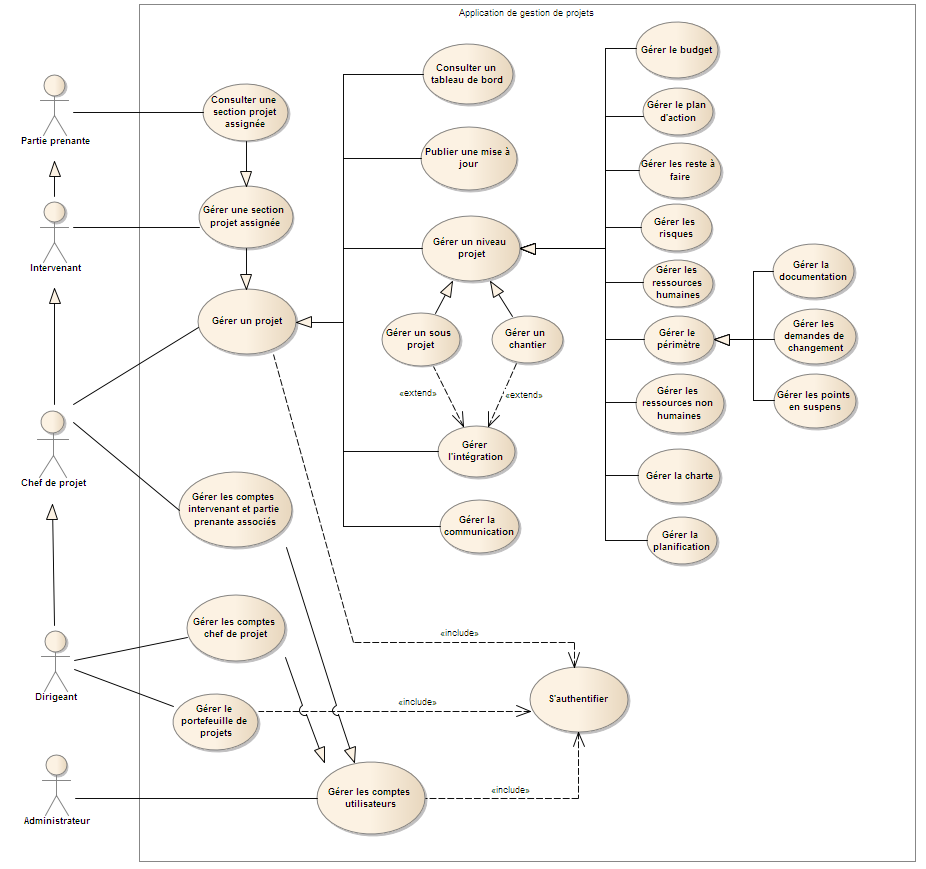
\includegraphics[width=1\linewidth]{useCasesDiag.png}
\caption{Diagramme global de cas d'utilisation}
\label{fig:useCasesDiag}
\end{figure}


%==============================================================================
\section{Étude technique}
Avant d'entamer la phase de développement, il est nécessaire de prendre du recul par rapport aux exigences et d'établir une vue d'ensemble du système d'un point de vue architectural. Dans notre cas en particulier, l'aspect SaaS de l'application impose une étude approfondie de l'infrastructure sous-jacente à mettre en place et des technologies à employer.

%-----------------------------------------------------------------------------------
\subsection{Architecture générale}
Une vue d'ensemble de l'architecture permet de mettre en évidence les différentes couches du système à développer.\\
Au vu du caractère Web de l'application, nous nous sommes d'abord orientés vers une architecture traditionnelle en 3-tiers \ref{3_tiers}, pour finalement opter pour une architecture en 4-tiers, se démarquant par l'ajout d'un serveur statique, séparé du serveur d'application, dédié à la récupération du front-end. Le schéma de la figure \ref{fig:baseArchitecture} illustre la relation entre les différents composants de cette architecture.

\begin{figure}[h]
\centering
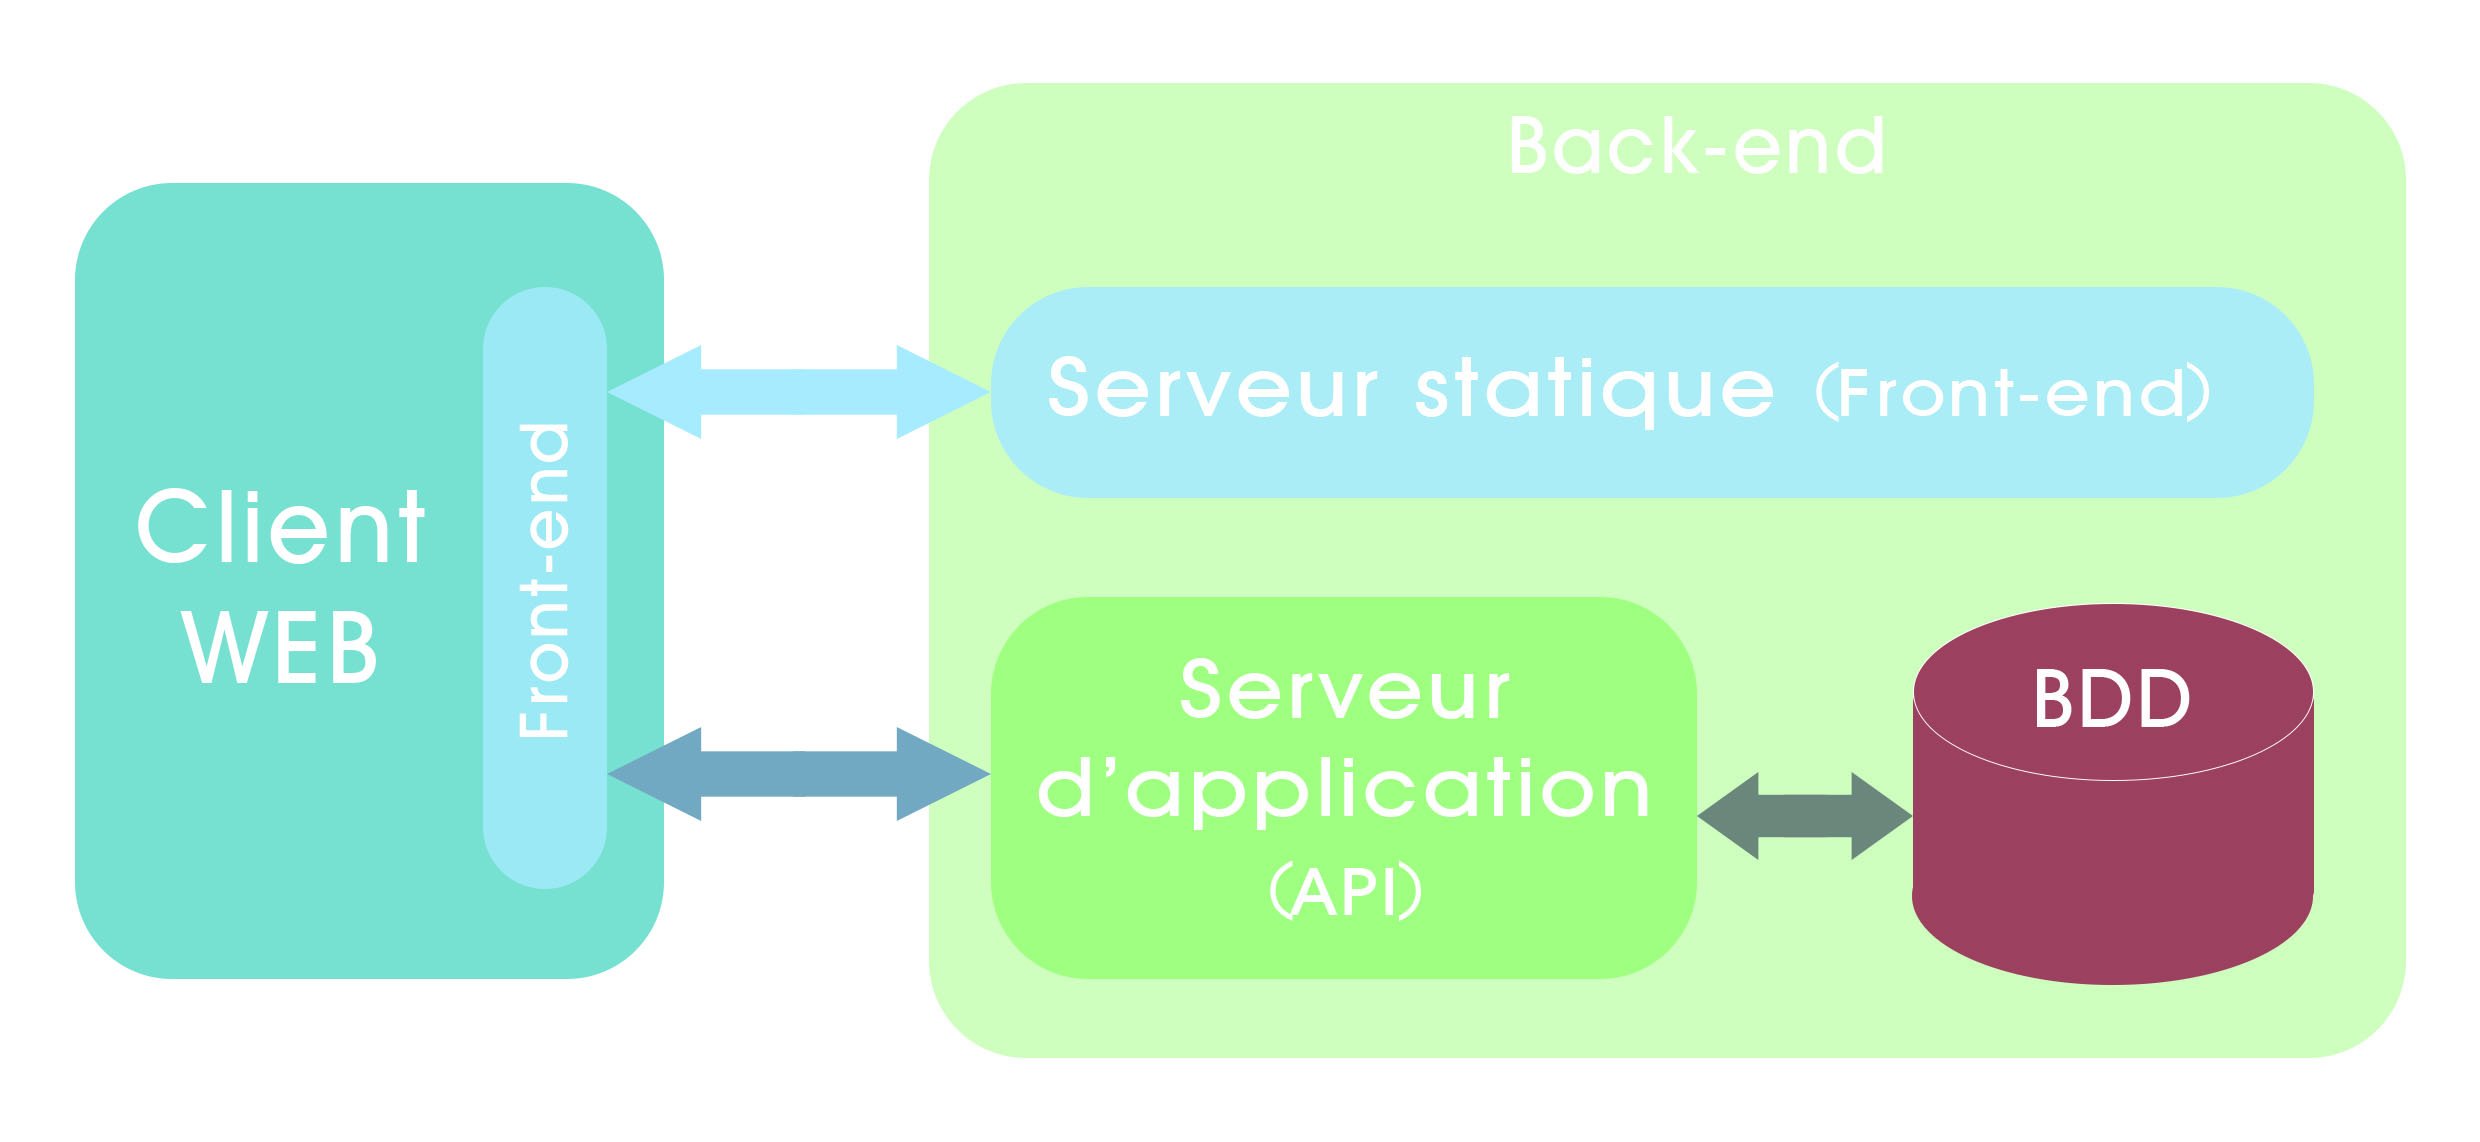
\includegraphics[width=1\linewidth]{baseArchitecture.jpg}
\caption{Architecture physique du système}
\label{fig:baseArchitecture}
\end{figure}
\

Notre système modélisé par le Back-end, chaque tiers représente l'une de ses couches. L'architecture logique du système se retrouve divisée en trois couches :
\begin{itemize}
    \item La couche d'accès aux données : Cette couche a pour charge la gestion des données du système (stockage, persistence, gestion de l'accès, ...).\\
Elle est représentée par notre base de données.
    \item La couche métier : C'est la partie fonctionnelle du système. Elle implémente la logique opératoire métier et se repose sur les données fournies par la couche inférieure. Elle offre des services à destination de la couche de présentation.\\
Elle est représentée par notre serveur d'application, qui fournit ces services sous forme d'un API.
    \item La couche de présentation : Elle encapsule l'interface utilisateur et correspond à la partie visible de l'application. Cette couche se repose sur les services offerts par la couche métier pour traiter les requêtes de l'utilisateur et s'occupe de la restitution et de la mise en forme des informations récupérées.\\
Elle est représentée par notre serveur statique, qui fournit l'application front-end au client.
\end{itemize}
\

Dans notre contexte, cette architecture en couches est la plus appropriée. L'architecture 3-tiers traditionnelle permet de bénéficier de :
\begin{itemize}
    \item Une répartition claire des responsabilités entre les couches
    \item Un couplage faible entre les différents niveaux
    \item Une simplicité lors de la réalisation de tests (la logique métier est isolée du reste des couches)
    \item Sécurité accrue, due à la séparation entre le client et les données
    \item La possibilité d'utilser des clients légers (adaptés aux dispositifs mobiles)
    \item Une évoluvité élevée, résultant de l'indépendance des couches
\end{itemize}
\

À partir de là, l'étape suivante logique pour une séparation plus aboutie des préopcupations, et donc une maintenance facilitée, a été l'orientation vers l'architecture en 4-tiers. Au travers de son adoption, nous avons clairement séparé entre l'application Front-end et l'application en charge de l'exposition de notre API. L'administration de ces deux applications sous la forme de deux projets distincts nous permet en plus de bénéficier de :
\begin{itemize}
    \item Un découplage net entre les rôles des deux applications
    \item Une évolution indépendante du Front-end
    \item Un déploiement séparé pour les deux applications
    \item Une montée en charge optimisée pour chaque entité
    \item Un versioning à part pour les deux projets
\end{itemize}
\

Les détails techniques de l'architecture seront exposés au cours des sections suivantes.

%-----------------------------------------------------------------------------------
\subsection{Technologies de base}
Pour traiter efficacement l'aspect SaaS du produit, un choix judicieux des technologies a été effectué préalablement au démarrage de la phase de développement. Nous procéderons à la présentation des technologies de base relatives à chacune des couches de notre architecture ainsi qu'à notre environnement de développement.

\subsubsection*{Couche de présentation}%--------------------------------------------------------------------------------
Pour réussir à développer un produit SaaS de qualité, on s'est orienté vers la mise en place d'une SPA (Single Page Application) pour la partie Front-end de notre application.\\

Dû à sa notoriété et à notre familiarité avec lui, le framework AngularJS a été notre choix de référence. L'ampleur de la communauté active développée autour de lui ainsi que l'abondance des ressources associées et le succès notoire en soi du framework nous a convaincu à l'adoption du framework en tant que brique de base pour le développement de la couche Front-end.

\subsubsection*{Couche métier}%-----------------------------------------------------------------------------------------
La couche métier de notre application nécessite le développement d'un API, dont les services seront exposés à la couche supérieure.\\
Vu les fonctionalités axées données (ressources) de notre application, nous nous sommes tournés vers la mise en place d'un API REST. En effet, dans notre cas, REST \ref{ANAGRAMME: REST} présente les avantages suivants :
\begin{itemize}
    \item L'adoption du standard HTTP en tant que protocole de communication. Son support universel assure une indépendance des technologies avec lesquelles intéragit l'API et ne restreint aucunement l'évoluvité du reste des composants.
    \item L'aspect sans état (stateless) du protocole facilite considérablement la montée en charge, considération importante à prendre en compte pour toute application en mode SaaS.
    \item Ce protocole est aussi optimisé pour l'interopérabilité avec les navigateurs (mise en cache, codes d'erreurs standards, ...) : REST représente en elle même l'architecture du web.
    \item Les Web services REST sont légers, ce qui les rend adaptés à la consommation via des dispositifs mobiles à ressources restreintes, exigence non fonctionnelle de notre application.
    \item Le support du format JSON le rend particulièrement adapté à l'interopérabilité avec le langage Javascript, qui n'est autre que le langage de dévelopement de la logique Front-end.
    \item L'abondance des technologies permettant de développer des API REST de qualité, de manière très productive.
\end{itemize}
\

Vu le succès retentissant des projets de l'entreprise d'accueil se reposant sur le langage Java, ainsi que notre familiarité avec le langage, il a été convenu dès le départ de l'adopter pour le développement en Back-end de notre produit.\\
Pour l'édification de l'API REST, nous avons favorisé l'usage de technologies conuues. C'est ainsi que nous avons opté pour l'emploi de la suite Spring. Véritable framework pour la conception de bout en bout de solutions logicielles complètes en Java, Spring offre une panoplie d'outils pour assiter à la mise en place d'un API REST. Les technologies Spring employées seront présentées en détail au cours du chapitre \ref{chap: BACKEND}.


\subsubsection*{Couche d'accès aux données}%----------------------------------------------------------------------------
Pour répondre aux besoins de gestion de données de notre application, nous avons procédé à une étude approfondie des systèmes de gestion de base de données disponibles sur le marché, répondant aux critères d'exigence définis par l'entreprise d'accueil. Cette étude sera exposée durant la section \ref{section: choix SGBDR} et aboutira à la détermination de la base de données à choisir pour les besoins de la couche d'accès aux données.

\subsubsection*{Environnement de travail}%------------------------------------------------------------------------------
Pour les besoins de versioning de notre travail, nous nous sommes reposés sur la solution Git.\\
Git est un logiciel libre créé par l'auteur du noyau Linux. En 2016, il s’agissait du logiciel de gestion de versions le plus populaire utilisé \ref{(en) « Git 2.8.2 Popular Source Code Management System Released with Over 18 Bug Fixes », sur Softpedia, 2 mai 2016 (consulté le 2 mai 2016)}. Il se distingue par un système de gestion de versions décentralisé.\\
Le choix de ce système de gestion de versions est judicieux dans notre cas, car il permet de garder une version complète de l'historique d'un projet en local, ce qui s'avère très utile pour le développement continue au sein et hors de l'entreprise.\\

La gestion de la liste des articles de travail ou du "Backlog" a été réalisée à l'aide de l'outil Trello.\\
Trello est à la base un outil de gestion de projet en ligne, lancé en septembre 2011, et inspiré par la méthode Kanban. Ce dernier point le rend très adapté à la gestion agile requise.

%-----------------------------------------------------------------------------------
\subsection{Choix du système de gestion de base de données}
Le choix du système de gestion de base de données est une étape cruciale pour le succès d'une application de type SaaS. L'étude suivante vise à mettre en exergue les fondations du choix de la solution retenue.\\

\subsubsection{Spécifications}%----------------------------------------------------------------------------------------
Commençons tout d’abord par spécifier les critères majeurs auxquels le système de gestion de données devra se plier :
\begin{itemize}
	\item \textbf{Disponibilité en open-source} :la licence associée à son exploitation devra permettre un usage commercial, sans imposer de frais relatifs à son obtention ou le dévoilement du code source propre à notre application
	\item \textbf{Maturité} :être stable, éprouvé en milieu réel et prêt à la mise en production
	\item \textbf{Structuration de données} :permettre de modéliser convenablement les données à persister
	\item \textbf{Requêtage multidimensionnel} :être adapté au besoin principal d’aide à la décision à offrir via l’application
	\item \textbf{Isolation de données} :permettre la séparation efficace des données relatives à chaque organisation, en conservant une certaine aisance d’utilisation
	\item \textbf{Consistance de données} :garantir pour chaque organisation, à tout moment, la consistance de ses données (support, au minimum, des transactions intra-organisation)
	\item \textbf{Durabilité de données} :offrir une persistance de données sure et infaillible (mécanismes de résistance aux pannes, pas de perte de donnée admise)
	\item \textbf{Performance} :être optimisé pour la lecture tout en assurant un temps d’écriture raisonnable
	\item \textbf{Productivité} :offrir une documentation de qualité, plus ou moins exhaustive, et posséder des ressources communautaires utiles
\end{itemize}
\\
\\
Un autre aspect, relatif généralement aux applications de type SaaS, serait la :
\begin{itemize}
	\item \textbf{Scalabilité} : support de mécanismes de montée en charge
\end{itemize}
\\
Cependant, celui-ci n’a pas été estimé prioritaire pour le moment dû au nombre restreint d’utilisateurs prévu pour le proche futur. 
Le problème devrait-t-il se manifester ultérieurement, une décision plus optimale pourra être prise à ce moment pour le régler (fondamentalement, scalabilité verticale ou horizontale), compte tenu de l’envergure plus importante qu’aurait pris le projet et du nouveau contexte auquel il sera soumis.\\
Néanmoins, celui-ci a été mentionné pour trancher éventuellement dans le cas d’un dilemme dans le choix entre des solutions très similaires.

\subsubsection{Présentation des solutions étudiées}%-------------------------------------------------------------------
Parmi les systèmes de gestion de base de données disponibles sur le marché, quelques options ont retenu notre attention lors du choix des solutions à considérer. Étant donné le caractère open-source recherché, des solutions telles que OracleDB ou SQL Server n’ont pas été prises en compte.\\
Les solutions étudiées se classifient essentiellement en deux catégories :
\begin{itemize}
    \item Les bases de données relationnelles
    \item Les bases de données non-relationnelles
\end{itemize}
\

Les bases de données relationnelles ayant étét considérées pendant plusieurs décennies comme le de facto pour le développement d’applications, deux solutions open-source se sont distinguées par rapport aux autres :
\begin{itemize}
    \item[•] \textbf{MySQL / MariaDB} :\\
C’est un système de gestion de bases de données relationnelles (SGBDR). Il fait partie des SGBDR les plus utilisés au monde, autant par le grand public (applications web principalement) que par des professionnels. Une partie de sa popularité provient de son inclusion dans les packages LAMP (Linux, Apache, MySQL/MariaDB, PHP) et ses variantes. MariaDB est une branche de MySQL maintenue par son créateur original. Celle-ci a vu le jour suite à l’acquisition de Sun (alors propriétaire de MySQL) par Oracle. À ce jour, leurs fonctionnalités restent très similaires. Il est développé dans un souci de performances élevées en lecture, ce qui signifie qu'il est davantage orienté vers le service de données déjà en place que vers celui de mises à jour fréquentes et fortement sécurisées.
    \item[•] \textbf{PostgreSQL} :\\
PostgreSQL est un système de gestion de base de données relationnelle et objet (SGBDRO). Ce système, concurrent d'autres systèmes de gestion de base de données libres ou propriétaires, est plus avancé que ses concurrents dans la conformité aux standards SQL et est pratiquement conforme aux diverses normes ANSI SQL. Il est largement reconnu pour son comportement stable, proche d’Oracle, mais aussi pour ses possibilités de programmation étendues, directement dans le moteur de la base de données.
\end{itemize}
\

D’une autre part, les bases de données non-relationnelles étant très populaires lors de la mise en place d’applications de type SaaS, les solutions suivantes ont aussi été considérées :
\begin{itemize}
    \item[•] \textbf{MongoDB} :\\
C’est un système de gestion de base de données orientée documents, répartissable sur un nombre quelconque d'ordinateurs et ne nécessitant pas de schéma prédéfini des données. Il est développé depuis 2007 par 10gen, devenue MongoDB. Le serveur et les outils sont distribués sous licence AGPL. Il fait partie de la mouvance NoSQL.
    \item[•] \textbf{Cassandra} :\\
C’est un système de gestion de base de données (SGBD) adhérant au mouvement NoSQL, conçu pour gérer des quantités massives de données sur un grand nombre de serveurs, assurant une haute disponibilité en éliminant les points individuels de défaillance. Initialement développée par Facebook, l'application a été libérée dans l'espace open source en juillet 2008. Le projet est maintenant porté par la fondation Apache.
    \item[•] \textbf{CouchDB} :\\
Apache CouchDB est un système de gestion de base de données orienté documents, écrit en langage Erlang, donc optimisé pour la concurrence et les environnements faibles en ressources. Il est distribué sous licence Apache. Conçu pour le Web, il fait partie de la mouvance NoSQL, et a été construit de manière à pouvoir être réparti sur de multiples serveurs.
\end{itemize}
\

Il est à noter que les solutions, dites « NoSQL », orientées clé-valeur n’ont pas été considérées, vu le manque de fonctionnalités (intentionnel) généralement offert. De même, la complexité des solutions orientées graphes ne parait pas justifiée face aux besoins de l’application.

\subsubsection{Comparatif}%-----------------------------------------------------------------------------------------
Le Tableau à la figure \ref{fig:comparatifDB} résume globalement la compatibilité des solutions considérées avec les spécifications établies précédemment.
On emploiera l’échelle illustrée par la figure\ref{echelleComparatifDB} pour comparer la richesse du support relativement à la fonctionnalité examinée :  de l’absence de support ou d’incompatibilité (1), jusqu’à un support optimal ou une richesse élevée de la granularité du support (5).
\begin{figure}[h]
\centering
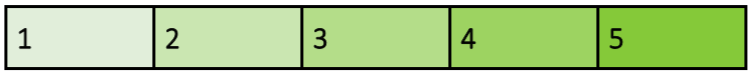
\includegraphics[width=0.5\linewidth]{echelleComparatifDB.png}
\caption{Échelle associée au tableau de la figure \ref{fig:comparatifDB}}
\label{fig:echelleComparatifDB}
\end{figure}
\

\begin{figure}[h]
\centering
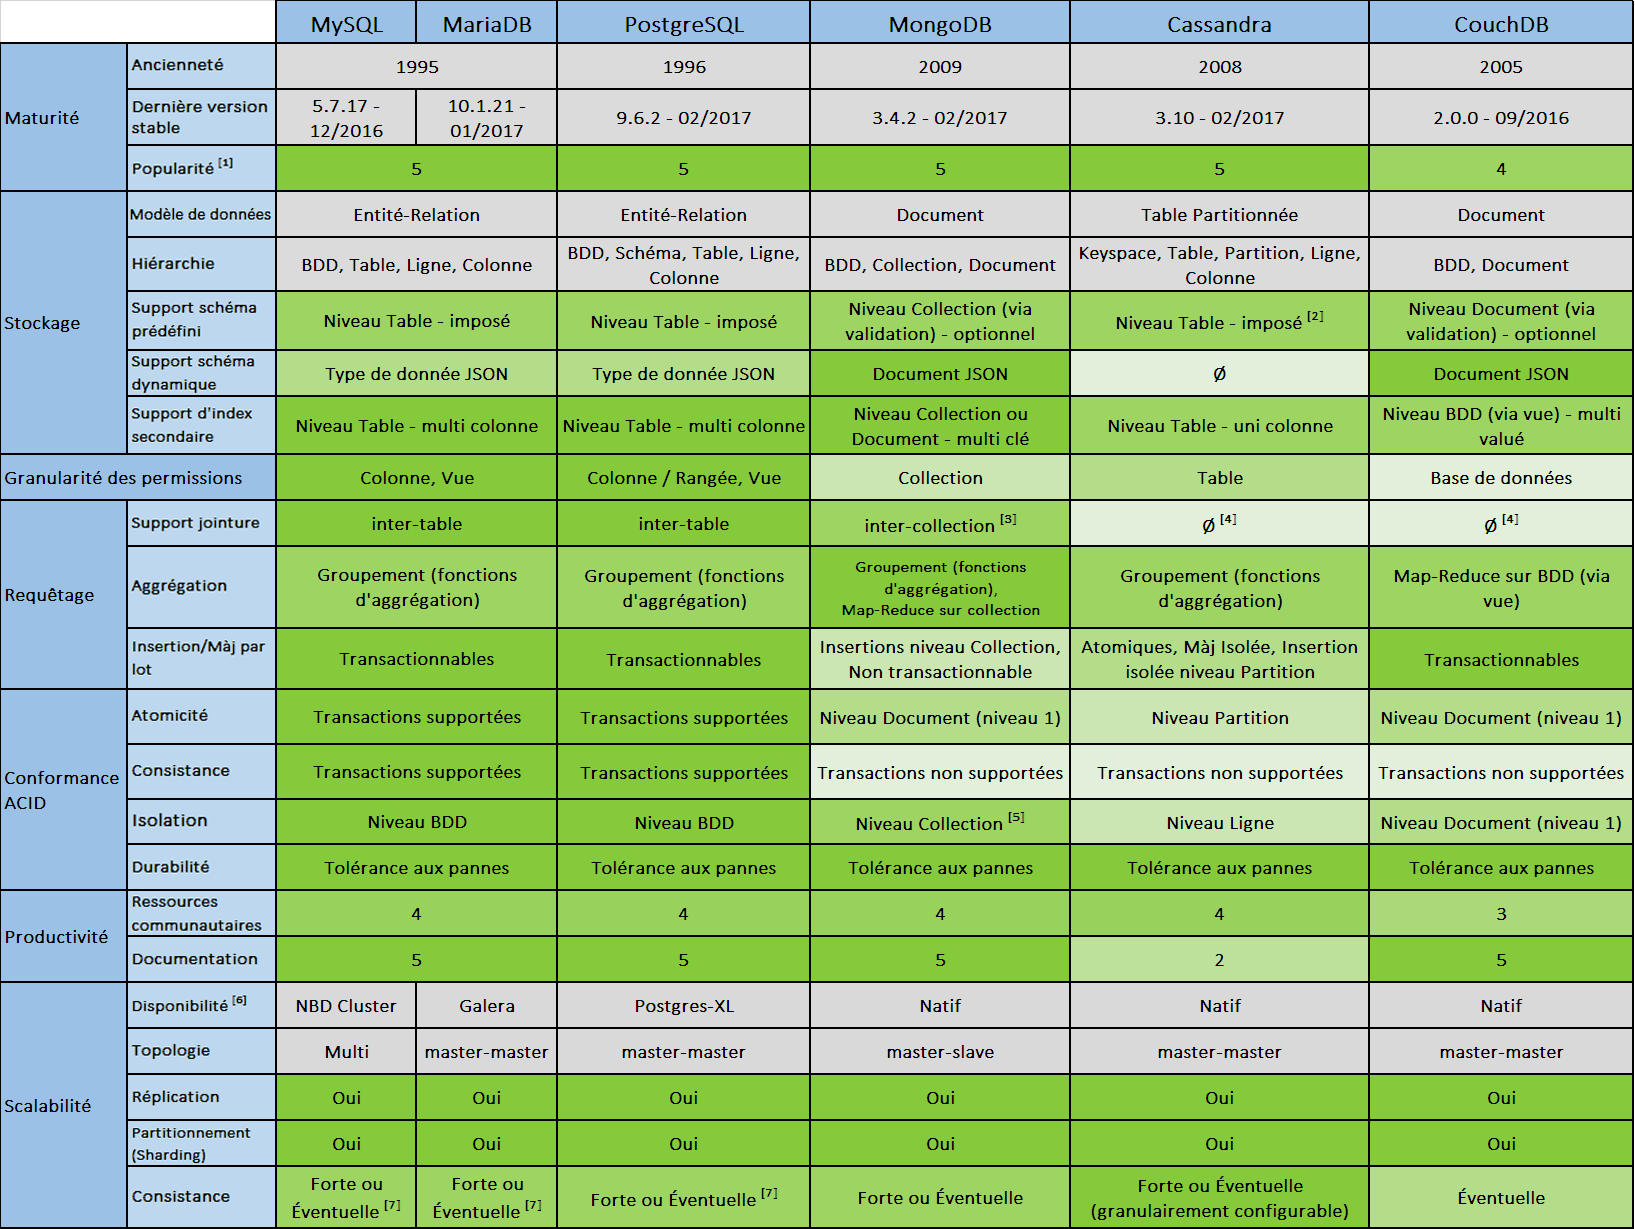
\includegraphics[width=1\linewidth]{comparatifDB.png}
\caption{Comparatif des solutions SGBDR considérées}
\label{fig:comparatifDB}
\end{figure}
\\
1 – Source: db-engines.com (Top10 = 5, Top20 = 4).\\
2 – Cassandra ne supporte plus les colonnes dynamiques (rendu obsolète par le remplacement de l’interface Thrift par CQL).\\
3 – Les jointures sous MongoDB ne sont supportés pour les données partitionnées (sharded).\\
4 – Cassandra et CouchDB ne supportent pas les jointures nativement. Cette fonctionalité est cependant possible avec SparkSQL ou le connecteur ODBC DataStax. Le concept de vue sous CouchDB permet de réaliser des un résultat comparable aux jointures, via des fonctions map-reduce.\\
5 – L’isolation sous MongoDB (uniquement via le mot clé $isolated) n’est pas supportées pour les données partitionnées.\\
6 – Pour les SGBDR, des solutions de montées en charge populaires ont été mis en avant pour la comparaison.\\
7 – La consistance (forte ou éventuelle) est gérée par le niveau d’isolation employé pour les SGBDR.\\

Les performances ne peuvent être concrètement évaluées que sous un benchmarking élaboré, propre aux besoins de notre application. Ce critère n’a en conséquent pas été traité dans le choix effectué. Il reste à noter que toutes les solutions offrent des performances raisonnables sous des conditions normales d'utilisation, d’après leurs communautés respectives.

\subsubsection{Bilan}%-----------------------------------------------------------------------------------------
On peut déduire du tableau que les solutions relationnelles supportent davantage les fonctionnalités à offrir à nos clients, étant hautement compatibles avec les besoins d’aide à la décision et de requêtage multidimensionnel. C’est surtout le support robuste des transactions et des jointures qui les favorisent par rapport aux autres solutions.\\
S'étant décidés à adopter une solution relationnelle, le choix final s’est porté sur PostgreSQL. Sa richesse en fonctionnalités et son support concret des schémas au sens SQL du terme, pour l’isolation des données, le place en tête par rapport à MySQL/MariaDB.\\
De plus, l’avenir de MySQL et de son alter-ego MariaDB, restant incertain quant à leur divergence éventuelle en fonctionnalités pour les versions futures, les pénalisent par rapport à PostgreSQL.\\

Notons toutefois que le développement de la couche d’accès aux données sera certainement réalisé à l’aide d’un middleware (ORM) qui permettra d’abstraire la base de données cible pour les déploiements internes, prévus de par la mise à disposition d’une offre alternative à l’offre SaaS (i.e on-premises). Dans un tel cas, une solution telle que MySQL pourra faire l’affaire malgré son manque de support concret des schémas, vu que le déploiement se fera pour une seule base de données (ou un nombre très restreint), le système traitant les schémas en tant que bases de données de manière sous-jacente.


%==============================================================================
\section*{Conclusion}
Ce chapitre a été l'occasion de prendre du recul par rapport au travail d'implémentation à réaliser. Les besoins de l'entreprise ont été formalisés et exprimés de manière explicite. Les fonctionalités requises du produit final identifiées, une étude technique a été entreprise en vue de poser les bases pour le travail de développement à effectuer.\\
Le dénouement de la phase d'inception annonce le début de la phase de construction. Cette phase sera détaillée en long et en large au cours des prochains chapitres.

%==============================================================================
\end{spacing}

\setcounter{chapter}{3}
\chapter{COUCHE FRONT-END}
\minitoc %insert la minitoc
\graphicspath{{Chapitre4/figures/}}

%\DoPToC

%==============================================================================
\pagestyle{fancy}
\fancyhf{}
\fancyhead[R]{\bfseries\rightmark}
\fancyfoot[R]{\thepage}
\renewcommand{\headrulewidth}{0.5pt}
\renewcommand{\footrulewidth}{0pt}
\renewcommand{\chaptermark}[1]{\markboth{\MakeUppercase{\chaptername~\thechapter. #1 }}{}}
\renewcommand{\sectionmark}[1]{\markright{\thechapter.\thesection~ #1}}

\begin{spacing}{1.5}

%==============================================================================
\section*{Analyse fonctionnelle}

%-----------------------------------------------------------------------------------
%\subsection{}


%==============================================================================
\section{Présentation des Frameworks et Patterns usités}


%==============================================================================
\section{Conception}


%==============================================================================
\section{Réalisation}


%==============================================================================
\section{Tests \& Validation}


%==============================================================================
\section*{Conclusion}


%==============================================================================
\end{spacing}

\setcounter{chapter}{4}
\chapter{          COUCHE BACK-END}
\minitoc %insert la minitoc
\graphicspath{{Chapitre5/figures/}}

%\DoPToC

%==============================================================================
\pagestyle{fancy}
\fancyhf{}
\fancyhead[R]{\bfseries\rightmark}
\fancyfoot[R]{\thepage}
\renewcommand{\headrulewidth}{0.5pt}
\renewcommand{\footrulewidth}{0pt}
\renewcommand{\chaptermark}[1]{\markboth{\MakeUppercase{\chaptername~\thechapter. #1 }}{}}
\renewcommand{\sectionmark}[1]{\markright{\thechapter.\thesection~ #1}}

\begin{spacing}{1.5}

%==============================================================================
\section*{Analyse fonctionnelle}

%-----------------------------------------------------------------------------------
%\subsection{}


%==============================================================================
\section{Présentation des Frameworks et Patterns usités}


%==============================================================================
\section{Conception}


%==============================================================================
\section{Réalisation}


%==============================================================================
\section{Tests \& Validation}


%==============================================================================
\section*{Conclusion}


%==============================================================================
\end{spacing}

\setcounter{chapter}{5}
\chapter{IMPLÉMENTATION DES SPÉCIFICATIONS NON FONCTIONNELLES}
\minitoc %insert la minitoc
\graphicspath{{Chapitre6/figures/}}

%\DoPToC

%==============================================================================
\pagestyle{fancy}
\fancyhf{}
\fancyhead[R]{\bfseries\rightmark}
\fancyfoot[R]{\thepage}
\renewcommand{\headrulewidth}{0.5pt}
\renewcommand{\footrulewidth}{0pt}
\renewcommand{\chaptermark}[1]{\markboth{\MakeUppercase{\chaptername~\thechapter. #1 }}{}}
\renewcommand{\sectionmark}[1]{\markright{\thechapter.\thesection~ #1}}

\begin{spacing}{1.5}

%==============================================================================
\section*{Analyse fonctionnelle}

%-----------------------------------------------------------------------------------
%\subsection{}


%==============================================================================
\section{Présentation des Frameworks et Patterns usités}


%==============================================================================
\section{Conception}


%==============================================================================
\section{Réalisation}


%==============================================================================
\section{Tests \& Validation}


%==============================================================================
\section*{Conclusion}


%==============================================================================
\end{spacing}

\setcounter{chapter}{6}
\chapter{          ASPECT SAAS}
\minitoc %insert la minitoc
\graphicspath{{Chapitre7/figures/}}

%\DoPToC

%==============================================================================
\pagestyle{fancy}
\fancyhf{}
\fancyhead[R]{\bfseries\rightmark}
\fancyfoot[R]{\thepage}
\renewcommand{\headrulewidth}{0.5pt}
\renewcommand{\footrulewidth}{0pt}
\renewcommand{\chaptermark}[1]{\markboth{\MakeUppercase{\chaptername~\thechapter. #1 }}{}}
\renewcommand{\sectionmark}[1]{\markright{\thechapter.\thesection~ #1}}

\begin{spacing}{1.5}

%==============================================================================
\section*{Analyse fonctionnelle}

%-----------------------------------------------------------------------------------
%\subsection{}


%==============================================================================
\section{Présentation des Frameworks et Patterns usités}


%==============================================================================
\section{Conception}


%==============================================================================
\section{Réalisation}


%==============================================================================
\section{Tests \& Validation}


%==============================================================================
\section*{Conclusion}


%==============================================================================
\end{spacing}



%%%%%%%% Figures

\makeatletter
%\renewcommand{a\thefigure}{\@arabic\c@figure}
\@addtoreset{figure}{chapter}
\makeatother

\renewcommand{\headrulewidth}{0.5pt}
\renewcommand{\footrulewidth}{0pt}
\renewcommand\listfigurename{Liste des Figures}
\listoffigures \mtcaddchapter

\fancyhead[R]{Liste des Figures}
\newpage


%%%%%%%% Tableaux

\makeatletter

\renewcommand{\headrulewidth}{0.5pt}
\renewcommand{\footrulewidth}{0pt}
\renewcommand\listtablename{Liste des Tableaux}

\listoftables  \mtcaddchapter

\fancyhead[R]{Liste des Tableaux}

%%%%%%%%%%%


\backmatter
\pagestyle{fancy}
\fancyhf{}
\renewcommand{\chaptermark}[1]{\markboth{Conclusion Générale et Perspectives}{}}
\fancyhead[R]{Conclusion Générale et Perspectives}
\fancyfoot[R]{\thepage}
\renewcommand{\headrulewidth}{0.5pt}
\renewcommand{\footrulewidth}{0pt}
%\chapter{Conclusion G�n�rale et Perspectives}
%==============================================================================
\pagestyle{fancy}
\fancyhf{}
\fancyhead[R]{\bfseries\rightmark}
\fancyfoot[R]{\thepage}
\renewcommand{\headrulewidth}{0.5pt}
\renewcommand{\footrulewidth}{0pt}
\renewcommand{\chaptermark}[1]{\markboth{\MakeUppercase{\chaptername~\thechapter. #1 }}{}}
\renewcommand{\sectionmark}[1]{\markright{\thechapter.\thesection~ #1}}

\begin{spacing}{1.5}
%==============================================================================

Dans une entreprise, la gestion des commandes re�ues est une �tape primordiale dans le processus, de conception et/ou de production. C'est l'�tape au cours de laquelle l'�coute du client est importante afin de bien comprendre ses besoins et de tenir compte de ses envies. Gr�ce � l'informatique, nous avons  pu r�pondre � cette probl�matique en utilisant le Customer Relationship Manager (CRM) qui est d�fini comme �tant l'ensemble des outils et techniques permettant de traiter et d'analyser toutes les informations relatives aux clients dans le but de les fid�liser en leur offrant les meilleurs services

Mais, comme toute solution, le CRM souffre d'un ensemble d'inconv�nients. Parmi eux, surgit le probl�me de la facilit� d'utilisation surtout pour les non-connaisseurs, comme les architectes. Nous avons donc pens� � une adaptation du concept du CRM aux besoins d'un architecte qui est une personne peu connaisseuse en informatique.
Dans ce cadre, nous avons effectu� ce stage de fin d'�tude dans la soci�t� � UrbaProd �. Nous �tions charg� de concevoir une plateforme de CRM qui permet, � la fois, de g�rer les demandes des clients en un laps de temps raisonnable, et de sauvegarder l'historique des diff�rentes demandes pass�es par le client. Notre plate-forme devra en plus �tre facile � utiliser par tous les utilisateurs, que ce soient des clients ou des architectes.
Afin d'atteindre ces objectifs, nous avons utilis� le "Framework" Symfony2. Il assure une grande performance et une facilit� d'extensibilit�, nous avons exploit� les composantes qu'il offre comme la gestion de s�curit� pour l'authentification et les droits d'acc�s.
A la fin de ce travail, nous avons r�pondu aux besoins de la soci�t� � travers l'ensemble des fonctionnalit�s fournies par notre solution, � savoir, le module de gestion des demandes, le module de notification et le module de gestion des clients.
Mais cela n'emp�che que nous avons connu quelques difficult�s pendant la p�riode de la collecte des besoins et des difficult�s pendant la p�riode de l'impl�mentation de la solution puisque l'entreprise ne comprend pas dans son effectif des sp�cialistes dans ce domaine.
L'utilisation de Symfony2 facilitera ensuite l'int�gration des am�liorations envisag�s par la soci�t� comme la notification par sms afin de garantir la visibilit� de l'information par tous les collaborateurs. M�me si nous avons utilis� des interfaces responsives, nous avons propos� d'impl�menter une application mobile qui sera plus ad�quate pour les smartphones.

%==============================================================================
\end{spacing} 


%\bibliographystyle{apalike-fr}
\bibliographystyle{Biblio/unsrt_modif}
%\singlespacing
\renewcommand{\bibname}{Bibliographie}

\bibliography{Biblio/aesm_edspia}

\onehalfspacing

\appendix
%\setcounter{figure}{0}
\setcounter{table}{0}
\setcounter{footnote}{0}
\setcounter{equation}{0}
\pagestyle{fancy}
\fancyhf{}
\renewcommand{\chaptermark}[1]{\markboth{\MakeUppercase{#1 }}{}}
\renewcommand{\sectionmark}[1]{\markright{\thesection~ #1}}
\fancyhead[RO]{\bfseries\rightmark}
\fancyhead[LE]{\bfseries\leftmark}
\fancyfoot[RO]{\thepage}
\fancyfoot[LE]{\thepage}
\renewcommand{\headrulewidth}{0.5pt}
\renewcommand{\footrulewidth}{0pt}

\makeatletter
\renewcommand\thefigure{A.\arabic{figure}}
\renewcommand\thetable{A.\arabic{table}}
\makeatother

\chapter{Annexe : Remarques Diverses - BIDON}
\graphicspath{{Annexe1/figures/}}
%==========================================================================

%    Annexe

%===========================================================================

\begin{figure}[!ht]
\centering

\includegraphics[scale=1]{ingenieur.jpg}
\caption{Demande sous sa forme originale}
\label{demOrgForm}
\end{figure} 


\end{document} 